%% This is a JAIR Example File Compiled by Nicholas Mattei (nsmattei@tulane.edu) 
%% and Odd Erik Gundersen (odderik@ntnu.no)
%% and Mykel Kochenderfer (mykel@stanford.edu)
%% September 15, 2025
%%
%% This file is based off the ACM Latex Template https://www.acm.org/publications/proceedings-template
%% Revision 2.12 (12/28/2024)
%% 
%% Please see https://www.jair.org/index.php/jair for more information and submission instructions.
%%

%% The first command in your LaTeX source must be the \documentclass
%% command.
%%
%% For submission and review of your manuscript please change the
%% command to \documentclass[manuscript, screen, review]{jair}.
%%
\documentclass[]{jair}


\setcopyright{cc}
\copyrightyear{2025}
\acmDOI{10.1613/jair.1.xxxxx}

% JAIR assigns the name of the AE (Associate Editor); authors leave this BLANK!
\JAIRAE{}  

% Insert JAIR Track Name only if part of a special track
\JAIRTrack{Integration of Logical Constraints in Deep Learning} 

\acmVolume{8x}
\acmArticle{6}
\acmMonth{8}
\acmYear{2026}

\RequirePackage[
  datamodel=acmdatamodel,
  style=acmauthoryear,
  backend=biber,
  giveninits=true,
  uniquename=init
  ]{biblatex}

\renewcommand*{\bibopenbracket}{(}
\renewcommand*{\bibclosebracket}{)}

%%
%% For managing citations, use BibLaTeX with the acmauthoryear style.
%% The next line specifies the bibliography file.
\addbibresource{my-nsai-kg.bib}


% ------------------------------------

\usepackage{graphicx}  % import graphics	

\usepackage{url}
\usepackage{listings}
\usepackage{threeparttable} % tables with captions and table notes
%\usepackage{booktabs}       % better tables (included in acmart.cls)

\usepackage{blindtext}
\usepackage{bussproofs} % for prooftree environment
\usepackage{amsmath}

\usepackage{xspace}  % used to build utility commands
\usepackage{todonotes}
\usepackage{enumerate}

% utility commands
\newcommand{\ie}{\textit{i}.\textit{e}.,\xspace}
\newcommand{\eg}{\textit{e}.\textit{g}.,\xspace}

\newcommand{\djh}[2][]{\todo[inline,bordercolor=blue,color=yellow!25, #1]{DH: {\footnotesize #2}}}

\newcommand{\ejr}[2][]{\todo[inline,bordercolor=blue,color=pink!25, #1]{EJR: {\footnotesize #2}}}

% ------------------------------------


%%
%% end of the preamble, start of the body of the document source.
\begin{document}

%%
%% The "title" command has an optional parameter,
%% allowing the author to define a "short title" to be used in page headers.
%\title{JAIR Example Template}
\title[KGR4VRD]{Logical Reasoning with OWL Knowledge Graphs for Learning and Validating Visual Relationship Detection}

%%
%% The "author" command and its associated commands are used to define
%% the authors and their affiliations.
%% Of note is the shared affiliation of the first two authors, and the
%% "authornote" and "authornotemark" commands
%% used to denote shared contribution to the research and/or corresponding author.
\author{David Herron}
\authornote{Corresponding Author.}
\orcid{0009-0008-2736-6789}
\email{david.herron@citystgeorges.ac.uk}
\affiliation{%
  \institution{City St George's, University of London}
  \city{London}
  %\state{British Columbia}
  \country{UK}
}

\author{Ernesto Jim\'{e}nez-Ruiz}
\orcid{0000-0002-9083-4599}
\email{ernesto.jimenez-ruiz@citystgeorges.ac.uk}
\affiliation{%
  \institution{City St George's, University of London}
  \city{London}
  %\state{British Columbia}
  \country{UK}}

\author{Tillman Weyde}
\orcid{0000-0001-8028-9905}
\email{t.e.weyde@citystgeorges.ac.uk}
\affiliation{%
  \institution{City St George's, University of London}
  \city{London}
  %\state{British Columbia}
  \country{UK}
}


%% The short list of authors must be made of the list of all authors' lastnames.
\renewcommand{\shortauthors}{Herron, Jim\'{e}nez-Ruiz \& Weyde}
%% If this is too long and overlaps other information printed in the page headers, use
%\renewcommand{\shortauthors}{Xu et al.}

%%
%% The abstract is a short summary of the work to be presented in the
%% article.
\begin{abstract}
{\bf Background:} 
    OWL (Web Ontology Language) knowledge graphs are not extensively used for knowledge representation and reasoning in neurosymbolic systems.  
    
    {\bf Objectives:}
    In this research, we demonstrate the benefits of performing OWL reasoning to guide and constrain deep (subsymbolic) learning in neurosymbolic systems. 
    
    {\bf Methods:}
    Our application domain is computer vision, specifically the task of visual relationship detection in images (VRD), for which we use our NeSy4VRD image dataset with its companion, common sense OWL ontology, VRD-World.
    We employ two OWL reasoning strategies, separately and in combination, to guide and constrain the subsymbolic learning and outputs of a multi-label classification neural network that predicts predicates of visual relationships (VRs) (\eg \texttt{person} \emph{on} \texttt{horse}, \texttt{person} \emph{ride} \texttt{horse}).
    Strategy 1 (annotation augmentation) uses deductive OWL reasoning to logically augment and enrich the annotated VRs (image scene graphs) that supervise the predicate learning, with the primary goal being to improve recall@N.
    Strategy 2 (prediction validation) uses OWL reasoning to identify predicted VRs that are semantically invalid according to VRD-World, \eg \texttt{person} \emph{drive} \texttt{horse}, with the primary goal being to minimise their number and thereby improve precision.
    Predictions identified as invalid by our OWL-based knowledge graph (acting as a real-time symbolic classifier) trigger semantic loss penalties during training, as \emph{soft} logical constraints, and are \emph{filtered-out} during inference, as \emph{hard} logical constraints.
    
    {\bf Results:}
    Our extensive evaluation shows the benefits of OWL representation and reasoning on the subsymbolic learning component, demonstrating the powerful capabilities of OWL-based knowledge graphs within a neurosymbolic system.
    
    {\bf Conclusions:}
    Our research introduces a new Semantic Web-based subcategory of the 'loss-based logical constraints' approach to neurosymbolic AI. It expands applications of OWL and OWL-based knowledge graphs by demonstrating their use as symbolic reasoning engines in neurosymbolic systems, where an OWL ontology (encoding common sense symbolic background knowledge) is used like a logic program to drive symbolic reasoning that guides and improves deep (subsymbolic) learning.
\end{abstract}

%% JAIR Note: 
%% Do not include ACM CCS Concepts or Keywords


%% To be updated by authors.
\received{3 October 2025}
\received[accepted]{tbd}

%%
%% This command processes the author and affiliation and title
%% information and builds the first part of the formatted document.
\maketitle

\section{Introduction}

Neurosymbolic AI has received increasing attention in recent years, and one approach to neurosymbolic AI focuses on using symbolic knowledge and logic to modulate the loss used to supervise deep (subsymbolic) learning, \eg \citet{DBLP:conf/nesy/SerafiniG16,DBLP:journals/jair/GiunchigliaL21,Giunchiglia2023}.
We describe research that establishes a novel Semantic Web-based subcategory of this `loss-based logical constraints' approach to neurosymbolic AI---research that leverages OWL-based knowledge graph reasoning to modulate loss and evaluate network outputs so as to guide and constrain subsymbolic learning.
\citet{DBLP:journals/semweb/HitzlerBES20} describe the promise of the role of the Semantic Web in neurosymbolic AI.
Our research demonstrates some of this promise.
It demonstrates the use of the Web Ontology Language (abbreviated OWL) \cite{OWL2:Primer}, via a custom OWL ontology expressing symbolic, common sense, background knowledge, and the use of available OWL-based knowledge graph infrastructure to provide logically sound and complete OWL reasoning services in neurosymbolic systems \cite{DBLP:conf/ore/MatentzogluLHSP15,DBLP:journals/corr/abs-2309-06888}.

The context of our research is the computer vision task of visual relationship detection (VRD) in images (scene graphs).
To study this task, we use our image dataset, NeSy4VRD \cite{Herron/2023/nesy4vrd}, whose images and high-quality visual relationship annotations are accompanied by a closely aligned, custom designed, common sense OWL ontology, VRD-World, that describes the domain of the dataset---a broad and sparse subset of common, everyday experience. 
NeSy4VRD is an enhanced version of the original VRD image dataset by \citet{lu2016visual}.
%\ejr{TODO: Briefly mention what our KG and ontology contains...}

Our baseline system encompasses both subtasks of VRD, but we focus here on the predicate detection subtask.
This is because our OWL ontology covers only relations between objects, not properties of individual objects.
Focusing on predicate detection allows us to study OWL reasoning on one level of the subsymbolic reasoning avoiding the complexities of multi-layered evaluation.

We explore two strategies for leveraging OWL reasoning in the predicate detection subtask of VRD. These two strategies are integrated with our baseline deep learning VRD system, leading to a neurosymbolic framework for VRD.
The first strategy, OWL reasoning strategy 1, involves \emph{annotation augmentation}.
We logically augment the visual relationships that have been annotated for the NeSy4VRD training images, and thereby logically enrich the targets that supervise the subsymbolic learning of our predicate detector.
The logical augmentation of the scene graphs is accomplished by leveraging OWL inference capabilities.
More specifically, strategy 1 focuses on \textit{symmetry}, \textit{inverse relationships}, \textit{transitivity}, \textit{property equivalence relationships}, and \textit{subproperty relationships}. We refer to these inference subcategories of OWL reasoning as \emph{OWL link inferences} as they infer \emph{implicit} links between individuals in an OWL-based knowledge graph.
We examine the differential effects on the subsymbolic learning of our predicate detector \emph{caused} by the activation of different OWL link inferences.
Each configuration enables OWL reasoning in a particular way, leading to different logical augmentations of the image scene graphs, and hence to different supervision for deep learning.

In strategy 2, \emph{prediction validation}, we use OWL reasoning to logically scrutinise predictions of visual relationships so as to classify them as logically valid or invalid according to our OWL ontology VRD-World.
The objective is to minimise the incidence of semantically invalid predicted visual relationships, which have no chance of being hits, and thereby help to improve precision (over baseline), and possibly recall@N as well.
Strategy 2 leverages \emph{OWL type inference} capabilities (where links between individuals and classes are inferred) and \emph{OWL consistency checking}  capabilities (where logical inconsistencies are~identified).

We apply strategy 2 OWL reasoning in our neurosymbolic VRD system during both predicate detector training and prediction.
During training, emerging predictions of visual relationships (composed of emerging predicate predictions for corresponding ordered pairs of objects) are proposed.
These new asserted visual relationships represent new facts and can be expressed as RDF triples \cite{RDFS/spec/2014} according to the vocabulary of the VRD-World ontology.
If the OWL reasoning gives rise to a logical inconsistency, when reasoning with VRD-World and the facts for a visual relationship, the visual relationship is tagged as invalid. 
Semantically invalid predictions attract semantic loss penalties, which are applied as \emph{soft} logical constraints, to steer the predicate detector away from them.
During inference, all predicted visual relationships are similarly classified as semantically valid or invalid. 
Here, however, relationships classified as semantically invalid are \emph{filtered out}, in the manner of \emph{hard} logical constraints, to \emph{guarantee} that zero semantically invalid predicted visual relationships emerge from the trained neurosymbolic VRD system.

This research demonstrates a variety of methods that contribute to neurosymbolic AI, all of which generalise well beyond the domain of visual relationship detection in images. 
With our proposed combination of OWL reasoning for augmentation and validation in neurosymbolic systems we make the following contributions, which we hope will encourage the community to engage with OWL knowledge graphs:
\begin{enumerate}[\it (i)]
 %\itemsep0.25em 
  \item We demonstrate the use of OWL-based knowledge graphs as symbolic reasoning engines in neurosymbolic systems.
  \item We demonstrate the effectiveness of OWL-based knowledge graph reasoning to help train and constrain a neural network classifier.
  \item We demonstrate the use of OWL-based \emph{soft}, \emph{hard} and \emph{implicit} logical constraints in neurosymbolic systems.
  \item We demonstrate the transfer of common sense, background knowledge (encoded in an OWL ontology) from the symbolic realm (of an OWL-based knowledge graph) to the subsymbolic realm of a neural network.
  \item We provide novel insights as to the effects on deep (subsymbolic) learning of different combinations of OWL link inferences.  
\end{enumerate}

This paper's companion GitHub repository contains code used in our research \cite{KGR4VRD_github}.
The NeSy4VRD image dataset and OWL ontology, VRD-World \cite{Herron/2023/nesy4vrd}, are on Zenodo~\cite{NeSy4VRD_v11}, and NeSy4VRD documentation and related sample code are on GitHub \cite{NeSy4VRD_github}.

The remainder of this paper is structured as follows.
In Section \ref{sec:preliminaries}, we discuss topics that form the background of our research.
Section \ref{sec:related-work} summarises categories of related work.
In Section \ref{sec:methods}, we detail our research methods.
In Section \ref{sec:evaluation}, we evaluate these methods by presenting and discussing the findings of our experiments.
Lastly, in Section \ref{sec:summary}, we summarise the ground covered, highlight our contributions, and describe potential future work.



\section{Preliminaries and background}
\label{sec:preliminaries}

Here we briefly discuss topics helpful for understanding the setting of our research.

\subsection{OWL-based Knowledge Graphs}
%
An ontology describes some domain of interest \cite{StaabAndStuder2009} in a standardised way, traditionally with the objective of facilitating precise communication and knowledge sharing using a logic formalism.
The Web Ontology Language (always abbreviated OWL) \cite{OWL2:Primer,Allemang2020,Uschold2018} is a key component of the W3C open standards ecosystem of the Semantic Web\footnote{RDF, RDFS and OWL are standards defined by the W3C: \url{https://www.w3.org/standards/}} \cite{SemanticWebBerners-Lee,Hitzler2010} and is currently the most extensively used language to define ontologies.
A prominent example is the public repository of ontologies BioPortal \cite{whetzel2011bioportal}.
OWL~2 is the current revision of the OWL Semantic Web language.
The formal underpinning of OWL~2 ontologies is based on the description logic $\mathcal{SROIQ}$ (refer to \citet{Baader2017,DBLP:conf/kr/HorrocksKS06} for an extensive description).

Knowledge graphs (KGs) are gaining increasing popularity in downstream applications. In its basic form, a knowledge graph conforms to a directed edge-labelled graph model, where nodes are concepts and entities of interest, and edges are relationships between them.
In this work, we rely on OWL-enhanced or OWL-based knowledge graphs, the most broadly accepted notion of knowledge graph within the Semantic Web~\cite{Hogan2021-KGBook}.
This type of KG is composed of RDF triples in the form \texttt{(h  p  t)}, where \texttt{h} represents the head or source of the triple (a class or an instance), \texttt{p} represents a predicate (a property), and \texttt{t} represents the tail or target of the triple (a class, an instance or a literal). 
KG entities (\ie classes, properties and instances) are represented by a URI (Uniform Resource Identifier). The prefixes \texttt{vrd:}, \texttt{rdf:}, \texttt{rdfs:} and \texttt{owl:}, for example, are namespace macros for base URIs that pertain to NeSy4VRD, RDF, RDFS and OWL, respectively. The names following the colons are appended to the base to create complete URIs. Thus, for example, \texttt{vrd:beside} is a compact (and conventional) way of referring to the URI  \url{http://www.semanticweb.org/nesy4vrd/ontologies/vrd_world#beside}.

An OWL-based knowledge graph can be split into triples defining the ontology or conceptual knowledge of the domain (\eg the custom-designed OWL ontology, VRD-World), and triples defining assertions or facts (\eg the annotated visual relationships in the NeSy4VRD dataset).
For example, the NeSy4VRD ontology, VRD-World, contains many categories of knowledge axioms expressed as triples.
It contains class subsumption triples such as \texttt{(vrd:Horse  rdfs:subClassOf vrd:Animal)}, object property characteristic triples such as \texttt{(vrd:beside rdf:type owl:SymmetricProperty)}, property relationship triples such as \texttt{(vrd:beside owl:equivalentProperty vrd:nextTo)} and \texttt{(vrd:over owl:inverseOf vrd:under)}, property domain restrictions such as \texttt{(vrd:drive rdfs:domain vrd:Person)}, and class disjointness triples such as \texttt{(vrd:Person owl:disjointWith vrd:Not\_Person)}.\footnote{Note that OWL also enables the creation of complex axioms that are translated/serialized into more than one triple: \url{https://www.w3.org/TR/owl2-mapping-to-rdf/}} 
The NeSyVRD visual relationship annotations, on the other hand, are interpreted as knowledge graph assertions or facts.
For example, we might refer to a generic NeSy4VRD visual relationship using the informal notation \texttt{(person ride horse)}.
But when referring to this visual relationship in the context of an OWL-based knowledge graph, we express the elements of the visual relationship as RDF triples, such as \texttt{(vrd:objectX vrd:ride vrd:objectY)}, \texttt{(vrd:objectY rdf:type vrd:Horse)}, and \texttt{(vrd:objectX rdf:type vrd:Person)}.

\subsection{OWL Reasoning}
OWL-based knowledge graph reasoning is supported by the available Semantic Web infrastructure, including OWL reasoners such as Pellet \cite{DBLP:journals/ws/SirinPGKK07}, ELK~\cite{KKS11:unchainel}, HermiT \cite{DBLP:journals/jar/GlimmHMSW14}, and RDFox \cite{DBLP:conf/semweb/NenovPMHWB15}.
Reasoning over large knowledge graphs using the full expressiveness of OWL may be prohibitively slow. 
For this reason, there is a specific profile of OWL~2 \cite{DBLP:conf/rweb/Krotzsch12}, OWL~2 RL, designed specifically to enable efficient reasoning over large knowledge graphs. OWL~2 RL has a direct translation into Datalog rules, enabling the use of efficient Datalog engines like RDFox.
Even though our research focuses on reasoning over tiny worlds (\ie image scene graphs, and individual visual relationships) rather than large knowledge graphs, all of the OWL reasoning conducted in our research was performed using the inference rules defined for OWL~2 RL.

Two kinds of entailments are leveraged in this study: \emph{OWL link inferences}, which derive new object property assertions (relations between individuals), and \emph{OWL type inferences}, which derive new class membership assertions (types of individuals). 
In particular, we focus on derivations by the following OWL constructs: symmetry (\texttt{owl:SymmetricProperty}), inverse relationships (\texttt{owl:inverseOf}), transitivity (\texttt{owl:TransitiveProperty}), property equivalence (\texttt{owl:equivalentProperty}) and subsumption (\texttt{rdfs:subPropertyOf}), class equivalence (\texttt{owl:equivalentClass}) and subsumption (\texttt{rdfs:subClassOf}), class disjointness (\texttt{owl:disjointWith}), and property domain (\texttt{rdfs:domain}) and range (\texttt{rdfs:range}) restrictions.
Below, we present examples of the inference rules (the inference semantics) associated with some of these OWL constructs, where the upper part denotes the premises, and the lower part the conclusion:\footnote{The complete set of inference rules defined for OWL~2 RL is available at: \url{https://www.w3.org/TR/owl2-profiles/}}

\begin{itemize}
    \item \textit{Symmetry (link inference):}

%\bigskip
%\noindent

\begin{footnotesize}
\begin{prooftree}
          \AxiomC{\texttt{(vrd:beside rdf:type owl:SymmetricProperty )}}  
          \AxiomC{\texttt{(vrd:objectX vrd:beside vrd:objectY)}}
          \BinaryInfC{\texttt{(vrd:objectY vrd:beside vrd:objectX)}}
\end{prooftree}
\end{footnotesize}

%\medskip
%\noindent
\item \textit{Inverses (link inference):}
\begin{footnotesize}
\begin{prooftree}
          \AxiomC{\texttt{(vrd:above owl:inverseOf vrd:below)}}  
          \AxiomC{\texttt{(vrd:objectX vrd:below vrd:objectY)}}
          \BinaryInfC{\texttt{(vrd:objectY vrd:above vrd:objectX)}}
\end{prooftree}
\end{footnotesize}


%\medskip
%\noindent
\item \textit{Class subsumption (type inference):}
\begin{footnotesize}
\begin{prooftree}
          \AxiomC{\texttt{(vrd:Dog rdfs:subClassOf vrd:Animal)}}  
          \AxiomC{\texttt{(vrd:objectX rdf:type vrd:Dog)}}
          \BinaryInfC{\texttt{(vrd:objectX rdf:type vrd:Animal)}}
\end{prooftree}
\end{footnotesize}


%\medskip
%\noindent
\item \textit{Domain restrictions (type inference):}
\begin{footnotesize}
\begin{prooftree}
          \AxiomC{\texttt{(vrd:ride rdfs:domain vrd:Person)}}  
          \AxiomC{\texttt{(vrd:objectX vrd:ride vrd:objectY)}}
          \BinaryInfC{\texttt{(vrd:objectX rdf:type vrd:Person)}}
\end{prooftree}
\end{footnotesize}

\end{itemize}


\subsection{OWL consistency checking}
In addition to link inference and type inference (which infer new facts), OWL reasoning can also identify logical inconsistencies that may arise as a consequence of the inference of new facts.
For example, if the relationship \texttt{(vrd:objectX vrd:ride vrd:objectY)} is predicted, and \texttt{objectX} has been classified as being a horse (and asserted with RDF triple \texttt{(vrd:objectX rdf:type vrd:Horse)}), this results in an inconsistency with respect to ontology VRD-World. The reason is that the domain of property \texttt{vrd:ride} is \texttt{vrd:Person}, which entails that \texttt{vrd:objectX} is a \texttt{vrd:Person}. Since \texttt{vrd:Horse} and \texttt{vrd:Person} are declared disjoint, an entity (\eg \texttt{vrd:objectX}) cannot be both a \texttt{vrd:Horse} and a \texttt{vrd:Person} simultaneously.
Additional examples are provided in Section \ref{sec:owl-reasoning-strategies}.

\subsection{Visual relationship detection}
Figure \ref{fig:vrd-in-a-nutshell} summarises the computer vision task of visual relationship detection (VRD) in images.
It also summarises the setting for our research into using external OWL-based knowledge graph reasoning to guide and constrain deep (subsymbolic) learning in neurosymbolic systems.
A visual relationship expresses a (binary) relationship between a particular ordered pair of objects in an image.
For example, Figure \ref{fig:vrd-in-a-nutshell} shows four visual relationships that have been annotated in relation to the dog and the surfboard objects in the associated image.
The top panel depicts a deep learning VRD system predicting two relationships in relation to the dog and surfboard, one of which matches with (hits) an annotated (target) visual relationship.
The bottom panel depicts a neurosymbolic system performing the very same task, with respect to the same pair of objects in the same image.
It expresses the hypothesis that, if the deep learning system leverages external, OWL-based knowledge graph reasoning, the neurosymbolic system can outperform deep learning by, \eg, generating more predictions, matching more of the annotated targets, improving precision, etc.

\begin{figure}
\center
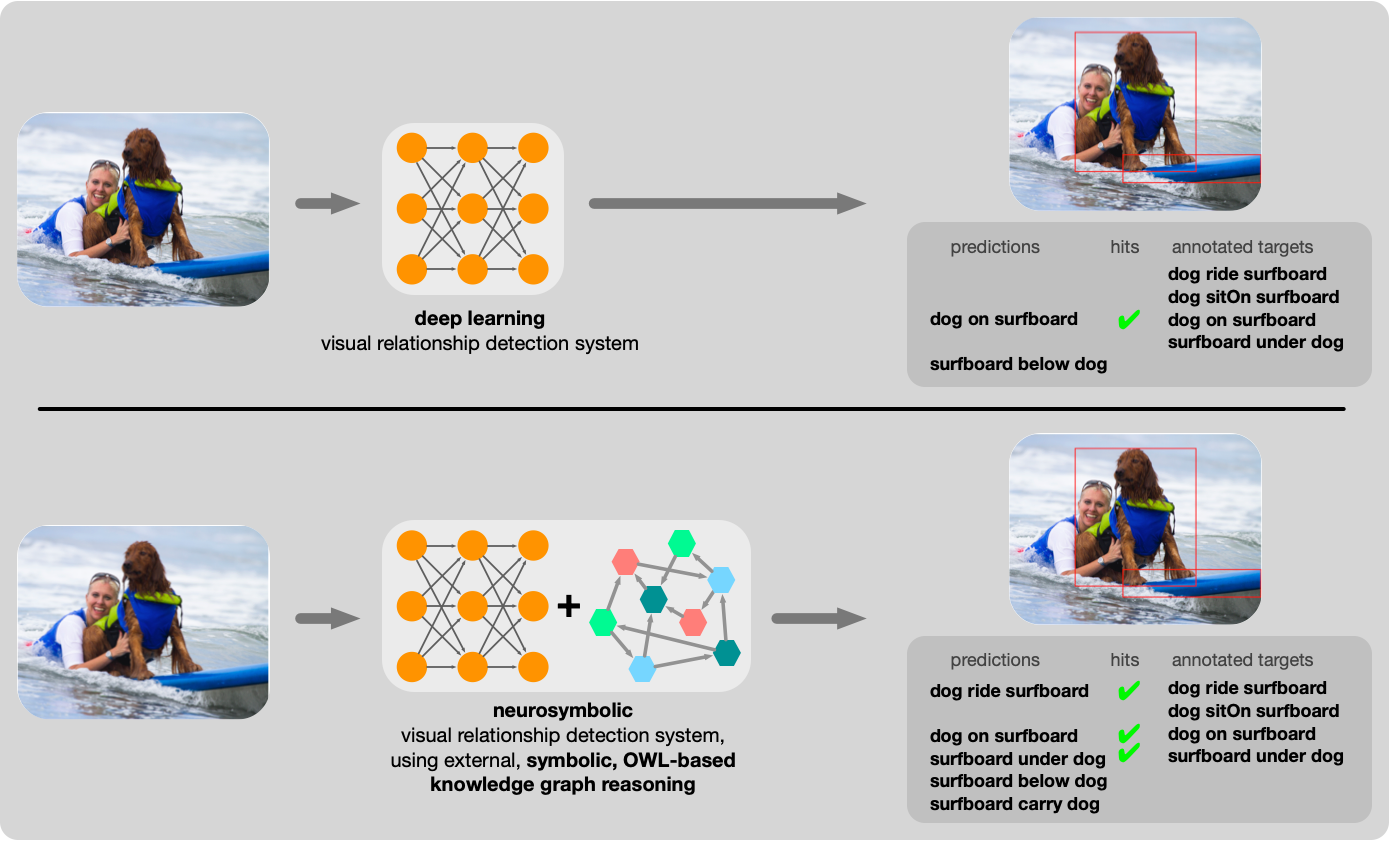
\includegraphics[width=0.8\textwidth]{figs/vrd-in-a-nutshell-v3.png}
\caption{\footnotesize A summary of the computer vision task of detecting visual relationships in images.  In the top panel, a deep learning system detects one of the four visual relationships annotated for a particular pair of objects in an image. The bottom panel expresses the hypothesis that a neurosymbolic system---one that uses external OWL reasoning to guide and constrain deep (subsymbolic) learning---can outperform deep learning by detecting more of the (ground-truth) visual relationships annotated for the image.}
\label{fig:vrd-in-a-nutshell}
\Description{An illustration of the computer vision task of visual relationship detection.}
\end{figure}

\subsection{NeSy4VRD}
The acronym NeSy4VRD stands for \emph{Neurosymbolic AI for Visual Relationship Detection}.
NeSy4VRD is a unique `image dataset plus OWL ontology' resource that we created to facilitate research into using OWL-based knowledge graphs in neurosymbolic systems for visual relationship detection.
It combines an image dataset, high-quality annotated visual relationships, and a companion, closely-aligned, common sense OWL ontology, VRD-World.
Such resources are so scarce we created our own.

NeSy4VRD is a successor to the VRD image dataset first introduced by \citet{lu2016visual}.
With permission from one of the principals behind that dataset, NeSy4VRD re-established public availability of the original VRD images---something which had disappeared some years prior due to server restructuring at Stanford University, where the dataset originated.
We found that the original visual relationships annotated for the VRD images suffered badly from the quality problems normally associated with crowd-sourcing.
These problems made design of a credible, companion OWL ontology infeasible.
They prompted us to undertake a major quality improvement exercise during which we extensively customised and comprehensively improved the quality of the annotated visual relationships.

In addition to the original VRD images, the NeSy4VRD quality-improved annotations, and the companion OWL ontology, VRD-World, NeSy4VRD includes all of the code and software infrastructure we developed in the process of cleaning the original VRD annotations (\eg extensive search services, a custom protocol for specifying annotation customisations declaratively in text files, and a configurable workflow for automating the application of annotation customisations in a controlled, repeatable fashion).
This infrastructure facilitates extensibility, and its availability invites researchers to extend and tailor NeSy4VRD (its annotations, and even the VRD-World ontology) for themselves and their particular research needs.
The dataset is relatively small (4000 training images, 1000 test images), and plenty of tooling is provided, so tailoring and extending NeSy4VRD for specialised needs may well be feasible for many researchers.

NeSy4VRD is described in detail in \citet{Herron/2023/nesy4vrd}.
The image dataset and its companion OWL ontology are available in the Zenodo repository \cite{NeSy4VRD_v11}.
The NeSy4VRD software infrastructure that supports the analysis and extensibility of NeSy4VRD itself, along with comprehensive documentation for how to use it, are available on GitHub \cite{NeSy4VRD_github}.


\subsection{The OWL ontology VRD-World}
The domain of the common, everyday images and annotated visual relationships of NeSy4VRD is a broad and sparse subset of the real world.
The image and the visual relationship annotations shown in Figure \ref{fig:vrd-in-a-nutshell} are representative.
In reference to this fact, we named the OWL ontology that we engineered to accompany the NeSy4VRD image dataset \emph{VRD-World}.
VRD-World is a custom-designed OWL ontology that describes the domain of the NeSy4VRD image dataset in a straightforward, common sense manner.
The alignment between the ontology and the image dataset is deliberately \emph{tight}, so that any OWL-based knowledge graph reasoning that takes place is pertinent to the subsymbolic learning task at hand.

More specifically, each of the 109 object classes of NeSy4VRD has a unique counterpart leaf class in the class hierarchy of VRD-World.
For example, the NeSy4VRD object classes \texttt{dog} and \texttt{cat} have corresponding VRD-World classes \texttt{vrd:Dog} and \texttt{vrd:Cat}, respectively.
These 109 leaf classes are unified by the common sense class hierarchy we designed for VRD-World.
For example, classes \texttt{vrd:Dog} and \texttt{vrd:Cat} are both declared to be subclasses of class \texttt{vrd:Carnivore} (a class unknown to NeSy4VRD).
And class \texttt{vrd:Carnivore} is declared to be a subclass of class \texttt{vrd:Mammal}, etc., to the top of the class hierarchy.
All of these parent classes are unknown to NeSy4VRD.

Similarly, each of the 71 predicates of NeSy4VRD (used to describe relationships between objects) has a unique corresponding OWL object property in VRD-World.
For example, the NeSy4VRD predicates \texttt{wear}, \texttt{behind}, and \texttt{hold} have counterpart OWL object properties \texttt{vrd:wear}, \texttt{vrd:behind}, and \texttt{vrd:hold}.
We inject further common sense, symbolic background knowledge into VRD-World by describing these object properties (these counterparts of NeSy4VRD predicates).
OWL object properties (binary relations) may be declared to possess a variety of characteristics and/or to be involved in various kinds of relationships with other object properties. 
For example:
\begin{itemize}
    \item property \texttt{vrd:nextTo} is declared to be a \emph{symmetric} binary relation, with OWL axiom \texttt{(vrd:nextTo rdf:type owl:SymmetricProperty)};
    \item property \texttt{vrd:over} is declared to have an inverse (property \texttt{vrd:under}), with OWL axiom \texttt{(vrd:over owl:inverseOf vrd:under)};
    \item property \texttt{vrd:below} is declared to be a \emph{transitive} binary relation, with OWL axiom \texttt{(vrd:below rdf:type owl:TransitiveProperty)};
    \item property \texttt{vrd:nextTo} is declared to be \emph{equivalent} to property \texttt{vrd:beside}, with OWL axiom \texttt{(vrd:nextTo owl:equivalentProperty vrd:beside)};
    \item and property \texttt{hold} is declared to be a \emph{subproperty} of property \texttt{vrd:touch}, with OWL axiom \texttt{(vrd:hold rdfs:subPropertyOf vrd:touch)}.
\end{itemize}

Table \ref{tab:onto-metrics} summarises OWL ontology VRD-World (version 1.2) by listing many of its key statistics, as calculated by the ontology editor Prot\'eg\'e~\cite{DBLP:journals/aimatters/Musen15}.
The original VRD-World (version 1.0) and the latest VRD-World (version 1.2) are available on Zenodo \cite{NeSy4VRD_v11}.
A comprehensive description of VRD-World (version 1.0) is provided in \citet{Herron/2023/nesy4vrd}.

\begin{table}[t]
\footnotesize
\caption{\footnotesize Summary statistics for OWL ontology VRD-World (version 1.2)}
\label{tab:onto-metrics}
\begin{center}
\begin{tabular}{l|r}
\toprule
\textbf{Summary metric} & \textbf{Count} \\
\midrule
Axioms & 1,103 \\
Logical axioms &  644 \\
Declaration axioms & 399 \\
Classes & 316 \\
Object properties & 74 \\
Data properties & 4 \\ 
Annotation properties & 10 \\
 \\
 \\
 \\
 \\
 \\
 \\
\bottomrule 
\end{tabular}
\quad
\begin{tabular}{l|r}
\toprule
\textbf{Class axioms} & \textbf{Count} \\
\midrule
SubClassOf & 319 \\
EquivalentClasses & 97 \\
DisjointClasses & 61 \\
\\
\toprule
\textbf{Object property axioms} &  \\
\midrule
SubObjectPropertyOf & 45 \\ 
EquivalentObjectProperties & 7 \\
InverseObjectProperties & 6 \\ 
TransitiveObjectProperties & 17 \\ 
SymmetricObjectProperties & 7 \\
ObjectPropertyDomain & 46 \\
ObjectPropertyRange & 23 \\
\bottomrule
\end{tabular}
\end{center}
\end{table}



% = = = = = = = = = = = = = = = = = = = = = = = = = = = = = = = = = =




\section{Related work}
\label{sec:related-work}


Here we point to categories of neurosymbolic systems research related to ours.
We mention a few representative examples for each one.
We also discuss one non-neurosymbolic research category that relates to our work.

\subsection{Visual relationship detection and scene graph generation}
The paper that introduced the VRD dataset, \citet{lu2016visual}, does not mention the notion of neurosymbolic, but the visual relationship detection system it describes can be seen as neurosymbolic since it relies upon word embeddings of the object class names and predicate names used in its annotations.
\citet{DBLP:conf/ijcnn/DonadelloS19} explore visual relationship detection on the VRD dataset using Logic Tensor Networks (LTN) \cite{DBLP:conf/nesy/SerafiniG16,DBLP:journals/ai/BadreddineGSS22}.
They describe using LTN \emph{Real Logic} knowledge axioms to declare \emph{negative domain} and \emph{negative range} constraints for relevant VRD dataset predicates.
Our OWL reasoning strategy 2 (prediction validation) can be viewed as a Semantic Web counterpart of their LTN-based strategy---one that declares (positive) domain and range restrictions for relevant object properties (NeSy4VRD predicates) in the OWL ontology VRD-World, and that uses OWL reasoning to enforce them (\ie to transfer knowledge of them to our predicate detector).

Some in the computer vision community speak of image scene graphs and scene graph generation rather than of visual relationships and visual relationship detection.
The survey by \citet{DBLP:journals/corr/abs-2201-00443} makes this clear.
It also shows that the VRD dataset has been a popular choice in scene graph generation research.
We use both forms of language.
As explained in \citet{DBLP:journals/internet/KhanBC22}, and in \citet{DBLP:journals/corr/abs-2201-00443}, scene graphs (or collections of visual relationships) are commonly used as precursors to a variety of enriched, downstream visual understanding and reasoning application tasks, such as image captioning, visual question answering, image retrieval, image generation, and multimedia event processing.

\subsection{Neurosymbolic AI using loss-based logical constraints}
The neural network training framework LTN \cite{DBLP:conf/nesy/SerafiniG16} uses one approach to blending logical constraints with loss functions in order to guide and constrain deep learning.
LTN requires a set of user-defined fuzzy logic knowledge axioms to be expressed that act as logical constraints to be satisfied. 
This set of axioms (this knowledge base) \emph{is} the loss function.
The network converges to the model that best satisfies the constraints \emph{in aggregate}.

\citet{DBLP:conf/nips/GiunchigliaL20} explore a different approach.
They present a neurosymbolic system that learns from externally specified symbolic background knowledge constraints that express simple implications that represent subClassOf relations between pairs of classes: \eg Dog $\rightarrow$ Carnivore, Carnivore $\rightarrow$ Mammal.
The objective is to teach a multi-label classifier the class hierarchy specified by the set of constraints (axioms) such that, if the network learns to predict that a datapoint (\eg fido) is a Dog, then it also learns to predict all of the parent classes of class Dog as well (\eg Carnivore, Mammal, Animal, etc.).
The problem itself is referred to as hierarchical multi-label classification (HMC).
The knowledge axioms are interpreted as logical constraints to be satisfied by the predictions of the classifier under training.
Constraints not satisfied that should be (\ie missing parent class predictions) attract loss penalties that guide the subsymbolic learning and convey the information about the class hierarchy.
\citet{DBLP:journals/jair/GiunchigliaL21} is an extension to \citet{DBLP:conf/nips/GiunchigliaL20} that also explores a generalisation of the HMC problem, where the axioms expressing relations between classes are more complex and more akin to the Horn clause inference rules used in logic programming.
\citet{HerronThesis2025} discusses explorations of the HMC problem using an architectural adaptation similar to the one employed by \citet{DBLP:conf/nips/GiunchigliaL20,DBLP:journals/jair/GiunchigliaL21}: we append one extra layer to a multi-label classifier, the size of the class hierarchy, so that it can handle the generalisation of base class predictions to their parent classes.
Rather than speaking of HMC, however, we speak of teaching a neural network the transitive closure of an OWL class hierarchy defined in an OWL ontology. 

Research based on the ROAD-R dataset \cite{Giunchiglia2023} develops this same approach outside the context of the HMC problem.
The ROAD-R dataset contains autonomous vehicle driving videos whose frames (images) have been annotated with the objects they contain.
The dataset supports visual relationship detection-type applications.
A set of 243 propositional logic `requirements' has been manually specified to accompany the dataset.
The requirements define admissible combinations of labels for 10 agent classes, 19 agent action classes, and 12 agent location classes: that is, logical conditions that should not arise, \eg a traffic light cannot be red and green at the same time.
If the network under training shows an inclination to predict something, a reasoner does a pass over this set of requirements to check that they are all satisfied.
If any are not satisfied, the prediction is of something inadmissible, and a loss penalty is computed and applied.

Our neurosymbolic research is conceptually closest to the approach taken by ROAD-R and the HMC-related work that precedes it.
Symbolic, background knowledge is expressed independently of the loss function---in our case, in an OWL ontology.
Via symbolic reasoning, the symbolic knowledge informs the calculation of loss, and leads to modulation of the loss signal, but the knowledge does not become the loss function itself, as with LTN.
In the case of ROAD-R, symbolic reasoning over the symbolic knowledge (the 243 propositional logic requirements) is undertaken using a SAT-solver.
In our case, OWL reasoners associated with OWL-based knowledge graph tools reason over the knowledge expressed in our OWL ontology, VRD-World.
Our approach can be viewed as a Semantic Web counterpart of the approach to `loss-based logical constraints' neurosymbolic AI used by ROAD-R.

\subsection{Knowledge graphs in neurosymbolic systems}
As interest in neurosymbolic AI research has grown, so has the frequency with which knowledge graphs feature as symbolic components in neurosymbolic systems~\cite{hitzlerKGinNSI2021/splncs}.
One example of this is the progressively developing theme of `deep deductive reasoning'~\cite{DBLP:conf/aaaiss/BianchiH19/iswc2022,DBLP:journals/apin/EbrahimiEBH21,DBLP:conf/aaaiss/EbrahimiSBXEDKH21/iswc2022}, where neural networks are trained to reason over knowledge graphs.
Knowledge graphs have been shown to be helpful in few-shot and zero-shot learning scenarios, where they help compensate for sparse training data, \eg \citet{Chen-Chen-Geng-ISWC-2021,DBLP:journals/semweb/GengCYYZC21,DBLP:journals/corr/abs-2112-10006/iswc2022}.
Knowledge graphs participate in Generative AI systems, where they are leveraged in RAG (retrieval augmented generation) schemes to enhance the context that augments LLM prompts in order to enhance LLM responses. 
The GraphRAG approach \cite{edge2025localglobalgraphrag} is a prominent example.

\subsection{OWL reasoning in neurosymbolic systems}
Despite the rising interest in using knowledge graphs in neurosymbolic systems, however, little neurosymbolic research uses OWL-based knowledge graphs, and even less does so in order to leverage OWL reasoning.
\citet{DBLP:journals/tgdk/dAmatoMMS23} note the scarcity of such research and remark that knowledge graph symbolic reasoning methods are under-explored and largely disregarded.
\citet{Breit-and-Waltersdorfer} conducted a systematic mapping study of 476 research papers that combine Semantic Web technologies with machine learning.
The study reports that only 20 (about 4\% of the total) mention using Semantic Web reasoning capabilities.
We consulted the study's companion online resource, the Semantic Web and Machine Learning Systems knowledge graph, or SWeMLS-KG \cite{DBLP:conf/esws/EkaputraLSEPBRWFA23}, and found 17 such papers.
Of these, we judge only~5 to use OWL reasoning (or 
related Semantic Web reasoning technologies) in some way.

These 5 papers share an important characteristic that aligns well with our research: the systems they describe all rely on the use of a \emph{custom} OWL ontology that was designed and tailored for the system at hand. 
\citet{DBLP:journals/access/ChangDGOSS20} describe a tutoring system that reacts  intelligently in response to interactions with human learners.
They leverage OWL \emph{type} inference capabilities---the ability for OWL reasoning to infer the classes to which individuals belong, in this case based on the attributes they possess (obtained via their interactions with the tutoring system).
\citet{DBLP:conf/semweb/DonadelloDE19} describe a digital healthcare system.
They supplement their custom OWL ontology with SPARQL rules \cite{Harris-SPARQL-2013}.
\citet{DBLP:conf/wetice/MouakherBBLHN19} describe a system for monitoring the bio-health of vineyards.
They supplement their custom OWL ontology with SWRL rules~\cite{Horrocks-SWRL-2004}.
\citet{DBLP:journals/cars/NakawalaBPCFM19} describe a system for recognising surgical processes for robot-assisted surgery.
They also supplement their custom OWL ontology with SWRL rules.
Fuller descriptions of these papers can be found in \citet{Herron/NAIJournal/2025}.

\subsection{Symbolic reasoning engines in neurosymbolic systems}
A subsymbolic learning system (of some kind) co-operating with an external symbolic reasoning engine (of some kind) is a particular \emph{pattern} of neurosymbolic system architecture (per, \eg \citet{DBLP:journals/jwe/HarmelenT19,DBLP:journals/apin/BekkumBHMT21,Breit-and-Waltersdorfer}).
The neurosymbolic system AlphaGeometry \cite{Trinh2024} is an instance of this pattern.
It combines a large language model (LLM) with a symbolic deduction engine.
Using Horn clause geometry rules, algebra rules, and associated inference algorithms, the LLM and the symbolic deduction engine co-operate in solving geometry problems. 
Similarly, systems built for the ROAD-R dataset \cite{Giunchiglia2023}, that use a reasoner to check whether propositional logic requirements (constraints) have been violated, are instances of this pattern.
Our research is another instance of the pattern.
In our case, however, the symbolic reasoning engine is an OWL-based knowledge graph hosting a custom OWL ontology.

\subsection{Automatic labelling}
Our OWL reasoning strategy 1 (annotation augmentation) relates indirectly to an area of machine learning research sometimes referred to as \emph{automatic labelling}, where strategies are explored for dealing with absences (or lack) of manually labelled data.
For example, \citet{DBLP:conf/soict/LeNN16} describe using a CNN to perform multi-label image annotation.
\citet{DBLP:journals/corr/abs-2203-01524}, however, opt instead to use semi-supervised learning to cope with their lack of labels, explaining that the quality of labels generated by automated means tends to be unreliable and problematic.
The logical augmentation of the image scene graphs that is central to our OWL reasoning strategy 1 can be viewed as being a form of automatic labelling extension.
In our case, however, the automatically generated (\ie inferred) visual relationships that augment the image scene graphs are reliably, logically sound---because the automatic generation mechanism is OWL reasoning.




% = = = = = = = = = = = = = = = = = = = = = = = = = = = = = = = = = =



\section{Methods}
\label{sec:methods}

In this section, we discuss our research methods.
We begin by describing our baseline deep learning system for visual relationship detection.
Then we describe our two OWL reasoning strategies.
First, we consider them from the theoretical perspective of the OWL logical inference capabilities that underpin them.
We map these capabilities to our two OWL reasoning strategies, and give examples to show how the strategies leverage the capabilities.
Then we consider our two strategies again, but this time from a systems perspective.
Here we explain, in turn, how each strategy integrates with the baseline deep learning system, and share operational details.
Lastly, we describe the metrics we use to assess the effects of OWL reasoning on guiding and constraining the subsymbolic learning of the predicate detector of the visual relationship detection system.

\subsection{Our baseline deep learning visual relationship detection system}
\label{sec:baseline-system}

\begin{figure}
\center
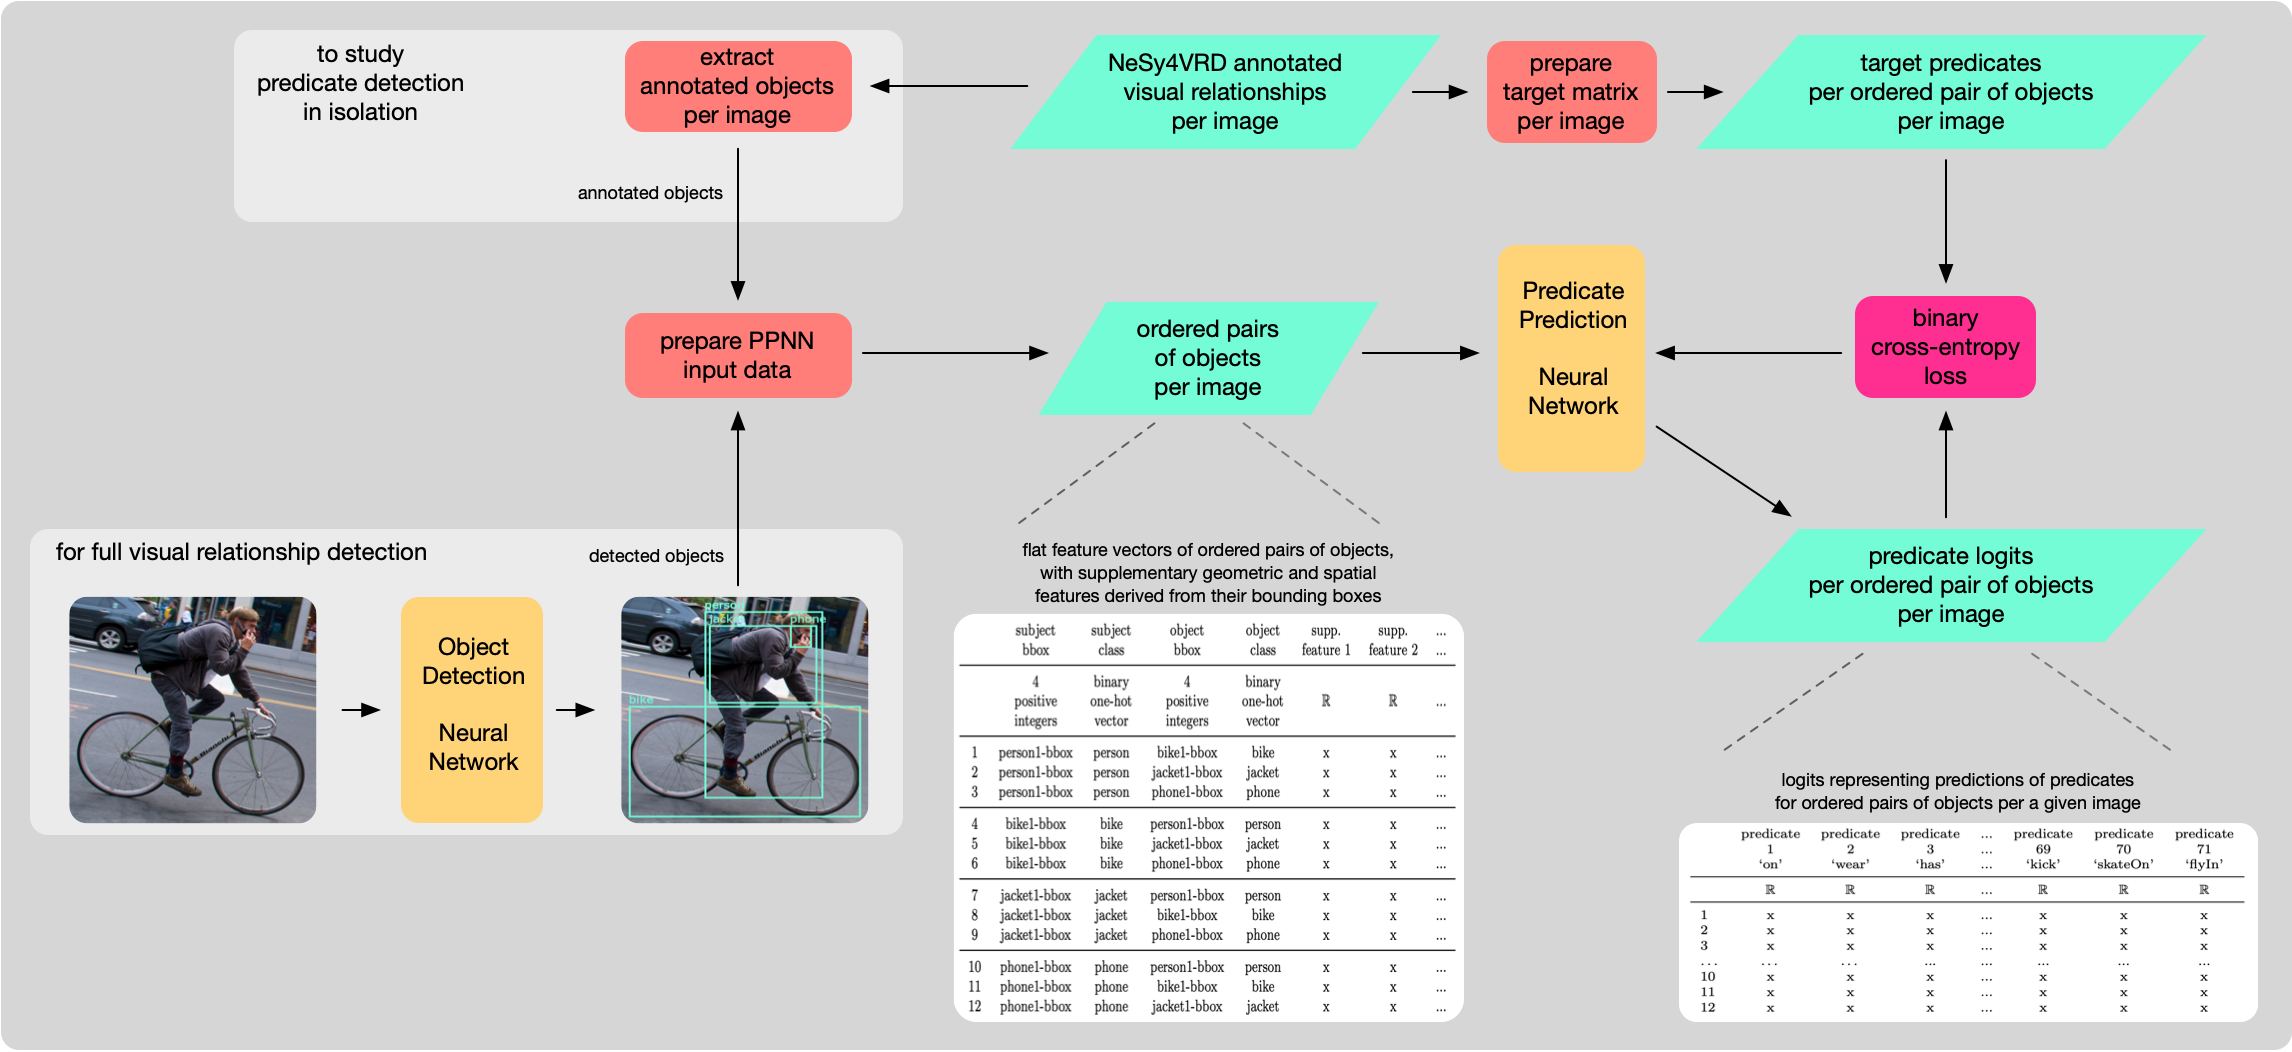
\includegraphics[width=1.0\textwidth]{figs/baseline-deep-learning-system5.png}
\caption{\footnotesize Our baseline deep learning system for detecting visual relationships. An object detection neural network detects objects in images, and a multi-label predicate prediction neural network predicts relationships between ordered pairs of those objects. To study the predicate detection aspect of visual relationship detection in isolation, the noise of the object detection can be cancelled by using (manually) annotated objects in place of (automatically) detected objects.}
\label{fig:architecture-baseline-system}
\Description{An illustration of our baseline deep learning visual relationship detection system. It distinguishes between the object detection and predicate prediction steps of the overall task, with a particular focus on showing the data inputs and outputs of our predicate prediction neural network.}
\end{figure}

Figure \ref{fig:architecture-baseline-system} describes the architecture of our baseline deep learning system for detecting visual relationships in images.
It is a simple pipeline of two neural networks: an object detection component followed by a predicate prediction component.
We discuss these two aspects of the system in turn.

\subsubsection{Object detection}
Following a convention first introduced by \citet{lu2016visual} with respect to their VRD dataset (the precursor of NeSy4VRD), and adopted by successive researchers (as is evident in the survey by \citet{DBLP:journals/corr/abs-2201-00443}), we distinguish between the task of full visual relationship detection (which includes object detection), and the subtask of predicate detection (which focuses on the prediction of relationships between objects).
One can cancel the noise introduced by the object detection (due to object misidentification) in order to study the predicate detection subtask in isolation. 
As explained earlier, the findings we present in Section \ref{sec:evaluation} pertain strictly to the predicate detection subtask because \textit{(i)} only our predicate detector (hereafter referred to as or predicate prediction neural network, or PPNN) is exposed to symbolic OWL reasoning, and \textit{(ii)} the cancellation of the object detection noise permits the effects on the subsymbolic learning of the PPNN to more clearly reveal themselves.
In recognition of this, instead of describing the object detection aspect of the baseline deep learning system here, we refer the reader to \citet{HerronThesis2025} where it is covered in detail.
The execution environment we describe there is as follows.
All object detection training and inference was undertaken using the PyTorch deep learning framework on the high performance computing (HPC) cluster at City St George's, University of London.
Each HPC compute node had 2 Intel Xeon Gold 6248R CPU processors, each processor having 24 cores, with 2 threads per core.
We used one NVidia A100 GPU and requested allocation of 4GB of GPU memory.
We used the PyTorch `cuda' device per the NVidia GPU.

\subsubsection{Predicate detection}
The predicate prediction neural network (PPNN) component of the baseline visual relationship detection system is a small feed-forward, multi-label classifier.
Its job is to predict predicates that describe relationships between objects.
Its four hidden layers, all linear, use an ELU activation function.
The output layer has no activation function, meaning the model returns raw logits.
The first three hidden layers are twice the size of the input feature vectors, and the fourth hidden layer is the size of the inputs.
The size of the output layer, 71, matches the number of predicates defined in NeSy4VRD.
In recognition of the fact that the PPNN is a multi-label classifier, when we convert logits to probabilities, we do so using a sigmoid function, not a softmax.
This architecture for our PPNN model proved to have the characteristics we sought: it showed itself to be a moderately capable learner---one capable of learning on its own, but not so capable as to leave no opportunity for symbolic OWL reasoning to add discernable value.

The reason our PPNN model is a \emph{multi-label} classifier is that it is common for NeSy4VRD images to have multiple visual relationships annotated for a given ordered pair of objects.
For example, here are two representative patterns:
\begin{itemize}
    \item \texttt{(person wear Y)}, \texttt{(person has Y)}, \texttt{(person in Y)}, where \texttt{Y} is some wearable thing, like a \texttt{shirt}, \texttt{jacket}, \texttt{jeans}, etc.;
    \item \texttt{(X beside Y)}, \texttt{(X nextTo Y)}, \texttt{(X adjacentTo Y)}, \texttt{(X near Y)}, where the predicates are synonyms or near synonyms of one another.
\end{itemize}

As shown in Figure \ref{fig:architecture-baseline-system}, as input the PPNN consumes flat feature vectors representing ordered pairs of objects.
Each object is represented by its bounding box (four integers) and a binary one-hot vector representing its class.
To help a PPNN learn, we supplement these core input features with a small number of geometric and spatial features derived from the bounding boxes of the ordered pair of objects.
For example, we compute the sine and cosine of the angle between the centroids of the two bounding boxes, and we compute two inclusion ratios that measure the extent to which one bounding box is included (contained) within the other.
We borrowed this idea for such supplementary geometric and spatial features from \citet{DBLP:conf/ijcnn/DonadelloS19}.

To train our PPNN models, we used binary cross-entropy loss.
During the training cycle, we did validation processing (on the NeSy4VRD validation set) in order to monitor predictive performance, which we measured using mean per image recall@50.
We saved model checkpoints at every epoch.
Our early-stopping mechanism used a patience of 25 epochs, and it always triggered in the range of 30 to 60 epochs.

For model selection, for the 35 latest PPNN checkpoint files (starting from the largest epoch number and working backwards) we performed inference on the NeSy4VRD test set.
For each checkpoint, inference was performed four times, each time with respect to one of four recall@N metrics, where $N \in \{25,50,100,999\}$.
The best performing model checkpoint file for each of the four recall@N metrics was then identified, where `best' is defined as the first model (\ie the one with the lowest epoch number) to deliver the maximum observed recall@N score.
Further details regarding predicate prediction are described in \citet{HerronThesis2025} and can be discerned in the source code available on GitHub \citet{KGR4VRD_github}.

With respect to execution environments, all predicate detection training and inference was undertaken using the PyTorch deep learning framework on consumer-grade computing infrastructure.
Experimentation was split across two similar platforms: \textit{(i)} a Mac Studio (M2 Ultra) desktop machine with 64 GB of memory and running macOS Sonoma, and \textit{(ii)} a MacBook Pro 16" (M2 pro) laptop machine with 16 GB of memory and running macOS Sonoma.
We used the PyTorch `mps' device in order to leverage the GPU \& Neural Engine features available on Apple Silicon platforms such as these.

\subsection{Our two OWL reasoning strategies - theory perspective}
\label{sec:owl-reasoning-strategies}

\begin{figure}
\center
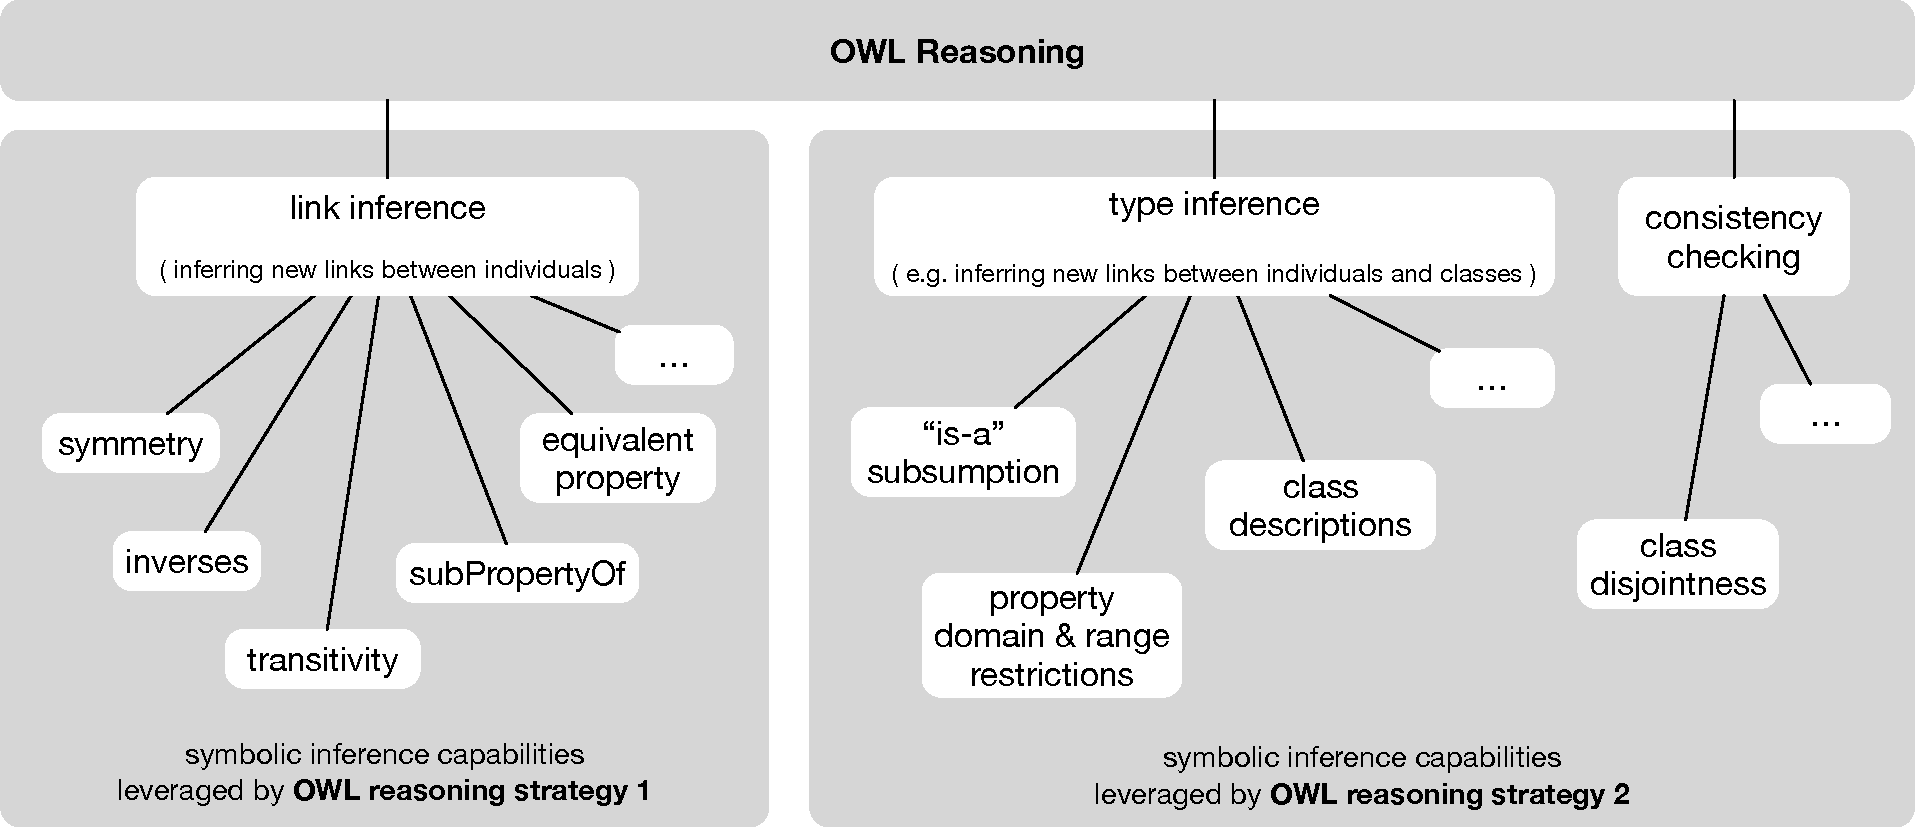
\includegraphics[width=0.9\textwidth]{figs/owl-reasoning-strategies-v4.pdf}
\caption{\footnotesize An informal summary and (partial) breakdown of the inference capabilities of OWL reasoning. The summary highlights the subcategories of OWL inference exercised in our research and maps them to one of our two OWL reasoning strategies. OWL reasoning strategy 1 (annotation augmentation) leverages OWL \emph{link} inference to logically augment image scene graphs by inferring new links between annotated objects. OWL reasoning strategy 2 (prediction validation) leverages both OWL \emph{type} inference and \emph{consistency checking} capabilities to classify predicted visual relationships as semantically valid or invalid. OWL \emph{link} and \emph{type} inference capabilities infer and materialise new knowledge (new RDF triples) in a knowledge graph. OWL \emph{consistency checking} detects logical inconsistencies but does not infer new knowledge.}
\label{fig:owl-reasoning-strategies}
\Description{A top-down, categorical decomposition of OWL reasoning, highlighting those of its logical inference capabilities used in our experiments. The first level of decomposition distinguishes between three categories of OWL reasoning capability: link inference, type inference, and consistency checking. The link inference category factors into the subcategories: symmetry, inverses, transitivity, subPropertyOf and equivalentProperty. The type inference category factors into: "is-a" subsumption, property domain and range restrictions, and class descriptions. The consistency checking category shows just one subcategory: class disjointness.}
\end{figure}

Figure \ref{fig:owl-reasoning-strategies} does an informal zoom-in on OWL reasoning in order to highlight the categories and subcategories of its inference capabilities that are exercised in our research.
It maps these capabilities to one of our two OWL reasoning strategies---strategy 1 (annotation augmentation), and strategy 2 (prediction validation)---to help the reader see the nature of the logical inference capabilities that underpin the two strategies.

For OWL reasoning strategy 1 (annotation augmentation), OWL \emph{link} inference capabilities are leveraged to enrich the training image annotated scene graphs by inferring new links (new relationships) between the annotated objects.
The axioms of OWL ontology VRD-World use OWL constructs that correspond to the five subcategories of link inference semantics highlighted in Figure \ref{fig:owl-reasoning-strategies}.
We arrange to activate different subsets (combinations) of these five subcategories of link inference semantics so that we can study their differential effects on the subsymbolic learning of our predicate prediction neural network (PPNN).
The entailment (or inference) rules defining the formal semantics associated with these different subcategories of link inference were detailed earlier, in Section \ref{sec:preliminaries}.

In contrast, for OWL reasoning strategy 2 (prediction validation), it is OWL's \emph{type} inference and \emph{consistency checking} inference capabilities that are exercised.
Taken together, these are what permit predicted visual relationships to be logically classified as being either semantically valid or invalid (according to VRD-World).
By \emph{type} inference, we refer to the capability of OWL reasoning to infer the classes to which individuals belong.
For example, a portion of the class hierarchy of OWL ontology VRD-World declares class \texttt{vrd:Dog} to be a subclass of class \texttt{vrd:Carnivore}, and \texttt{vrd:Carnivore} to be a subclass of \texttt{vrd:Mammal}.
Thus, when some individual is asserted to be a dog, with, say, an RDF triple such as \texttt{(vrd:objectX rdf:type vrd:Dog)}, OWL reasoning infers that \texttt{(vrd:objectX rdf:type vrd:Carnivore)} and \texttt{(vrd:objectX rdf:type vrd:Mammal)}.

OWL reasoning strategy 2 also leverages the fact that OWL permits properties to have their domains and ranges restricted.
The inference semantics of such restrictions lead to more OWL \emph{type} inference.
For example, VRD-World restricts the domain of property \texttt{vrd:wear} (NeSy4VRD predicate `wear') to members of class \texttt{vrd:WearCapableThing} (which is defined as the parent class of, among others, \texttt{vrd:Person}, \texttt{vrd:TeddyBear}, \texttt{vrd:Dog} and \texttt{vrd:Horse}).
If an RDF triple is asserted such as \texttt{vrd:objectX vrd:wear vrd:objectY}, then OWL reasoning infers that \texttt{vrd:objectX rdf:type vrd:WearCapableThing}.
The summary statistics for VRD-World reported in Table \ref{tab:onto-metrics} indicate that 46 object properties (counterparts of NeSy4VRD predicates) have had their domains restricted in some way, and 23 have had their ranges restricted in some way.

For each class referenced in an object property domain or range restriction, VRD-World contains a definition for a counterpart \emph{complement} class.
For example, the complement class of class \texttt{vrd:WearCapableThing} is class \texttt{Not\_WearCapableThing}.
Each pair of complement classes is declared to be \emph{disjoint}.
These declarations of disjoint classes create conditions that make it possible for OWL reasoning (in our case, OWL \emph{type} inference) to give rise to logical inconsistencies.

For example, let the following set of RDF triples represent a hypothetical predicted visual relationship that is inserted into our OWL-based knowledge graph hosting VRD-World (\ie our real-time symbolic reasoning binary classifier):%
\begin{verbatim}
vrd:objectX rdf:type vrd:Table .
vrd:objectY rdf:type vrd:Hat .
vrd:objectX vrd:wear vrd:objectY .
\end{verbatim}
The first RDF triple leads OWL \emph{type} inference to infer that \texttt{vrd:objectX} is of type \texttt{vrd:Not\_WearCapableThing}, because class \texttt{vrd:Table} is one of its subclasses (\ie in VRD-World, tables cannot wear things).
The third triple leads OWL \emph{type} inference to infer that \texttt{vrd:objectX} is of type \texttt{vrd:WearCapableThing}, because the domain of property \texttt{vrd:wear} has been restricted to class \texttt{vrd:WearCapableThing}.
The resulting situation, however, represents a logical contradiction (a logical inconsistency)---because classes \texttt{vrd:WearCapableThing} and \texttt{vrd:Not\_WearCapableThing} have been declared \emph{disjoint}, so no individual can be a member of both simultaneously.
The \emph{consistency checking} capabilities of OWL reasoning will detect this logical inconsistency.




\subsection{Strategy 1 (annotation augmentation) - systems perspective}
\label{sec:methods-strategy-1}

\begin{figure}
\center
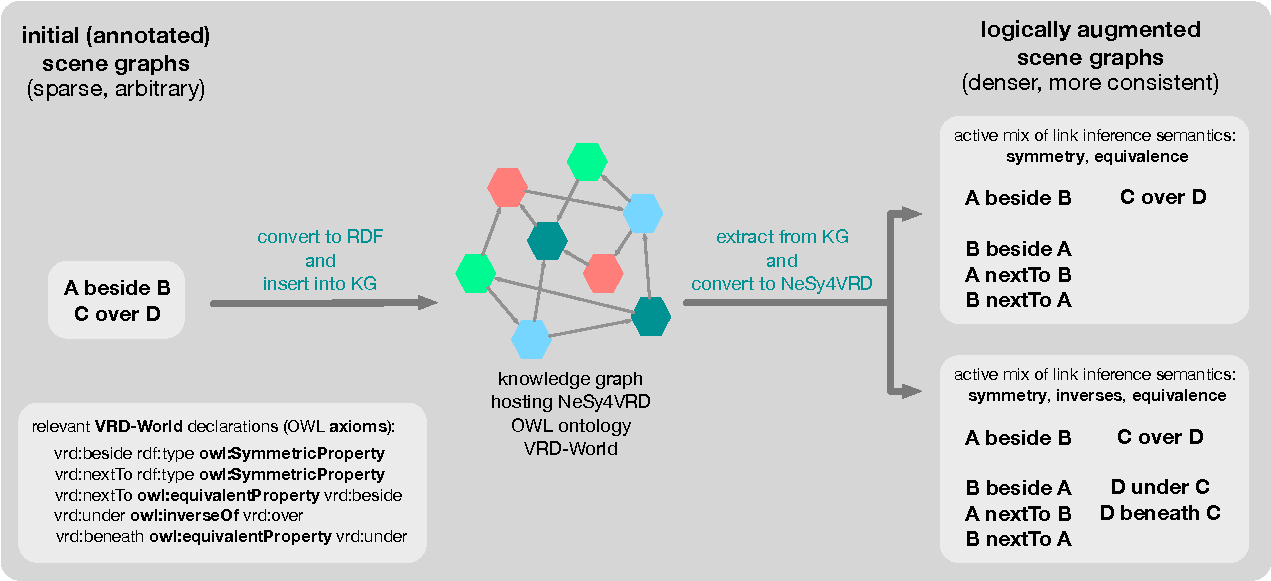
\includegraphics[width=\textwidth]{figs/nnkgs0-anno-aug-v3.pdf}
\caption{\footnotesize An illustration of OWL reasoning strategy 1, annotation augmentation, in action. The OWL-based knowledge graph hosting OWL ontology VRD-World acts as a symbolic reasoning engine. It logically augments the hypothetical (and deliberately simple) annotated training image scene graph on the left. The outcome of the logical enrichment varies (generally) depending on the subset (or mixture) of five subcategories of OWL \emph{link} inference semantics that are activated within VRD-World at the time of augmentation. The logically augmented scene graphs inferred by a given configuration of VRD-World are then used to supervise neural network training.}
\label{fig:nn-kg-s0-setting}
\Description{An illustration of our OWL reasoning strategy 1: annotation augmentation. An OWL-based knowledge graph hosting our NeSy4VRD OWL ontology, VRD-World, is in the centre.  A representative annotated scene graph (small and sparse) is input to the KG from the left, and the KG is shown generating different logical expansions of the input scene graph, according to activations of different mixtures of link inference semantics within OWL ontology VRD-World.}
\end{figure}

Figure \ref{fig:nn-kg-s0-setting} summarises OWL reasoning strategy 1 (annotation augmentation) pictorially.
An OWL-based knowledge graph hosting OWL ontology VRD-World is used as a symbolic reasoning engine to logically augment the (rather sparse and arbitrary) scene graphs annotated for the NeSy4VRD images.
The logically augmented scene graphs (for the given configuration of OWL ontology VRD-World that inferred them) are then used to supervise the training of the predicate prediction neural network (PPNN), as depicted earlier, in Figure \ref{fig:architecture-baseline-system} (the baseline deep learning visual relationship detection system).
When the component in the top row of Figure \ref{fig:architecture-baseline-system}---the one named `NeSy4VRD annotated visual relationships per image'---is replaced by a set of logically augmented visual relationships per image, then Figure \ref{fig:architecture-baseline-system} effectively represents a neurosymbolic system that corresponds to our OWL reasoning strategy 1.
The hypothesis underlying OWL reasoning strategy 1 is that logical augmentation of the training image scene graphs will enrich the supervision they afford to deep learning, and guide and constrain the subsymbolic learning of the PPNN component in ways that deliver improved predictive performance.

\begin{table}[t]
  \centering
  \footnotesize
  \begin{threeparttable}
  \caption{\footnotesize The meaning of the names for the treatments used to explore the effects of OWL reasoning strategy 1 (annotation augmentation) on subsymbolic learning. For OWL reasoning strategy 1, treatments are configurations of activated link inference semantics within OWL ontology VRD-World, and the corresponding neural network (PPNN) models that emerge from having been trained on target scene graphs logically enriched by OWL reasoning governed by that configuration of VRD-World.}
  \label{table:invest1-treatments}
  \begin{tabular}{llll}
    \toprule 
     treatment   & treatment  & mixture of activated & relevant Semantic Web \\
     name        &  key & OWL link inference semantics & (OWL) construct \\
    \midrule
    t01 & S\_\_\_\_  & symmetric properties & owl:SymmetricProperty \\
    t02 & \_I\_\_\_  & inverse relationships & owl:inverseOf  \\
    t03 & \_\_T\_\_  & transitivity properties & owl:TransitiveProperty \\
    t04 & \_\_\_E\_  & equivalence relationships & owl:equivalentProperty \\
    t05 & \_\_\_\_U  & subproperty relationships & rdfs:subPropertyOf \\
    t07 & \_\_\_EU  & t04, t05  \\
    t08 & \_\_TEU  & t03, t04, t05  \\
    t09 & S\_TEU  & t01, t03, t04, t05  \\
    t10 & SITEU  & t01, t02, t03, t04, t05  \\
    t11 & \_ITEU  & t02, t03, t04, t05  \\
    t12 & SI\_\_\_  & t01, t02  \\
    t14 & S\_\_E\_  & t01, t04  \\
    \bottomrule 
  \end{tabular}
  \end{threeparttable}
\end{table}

We could have opted to do the logical augmentation of the annotated training image scene graphs in real-time, during a PPNN training cycle, but since logical inference is deterministic, this approach would have involved much repetitive (and, hence redundant) inference, as each image is re-encountered in successive training epochs.
Thus, there were compelling practical reasons for performing the logical augmentation upfront, once, as part of a pre-processing step.
But use cases different from ours will surely exist where the inference to be performed is dynamic and must be performed in real-time.

In Section \ref{sec:evaluation}, where we present the findings associated with OWL reasoning strategy~1, we refer to the different configurations of VRD-World (the different subsets of activated link inference semantics), and to the trained neurosymbolic systems associated with them, as \emph{treatments}.
Table \ref{table:invest1-treatments} defines the various treatments we explored in connection with OWL reasoning strategy 1.

To perform the actual logical augmentation of the image scene graphs, we used the two open-source tools RDFLib\footnote{\url{https://github.com/RDFLib/rdflib}} and OWL-RL\footnote{For strategy 1, we used OWL-RL (\url{https://github.com/RDFLib/OWL-RL}) for simplicity, but other more sophisticated solutions like RDFox \cite{DBLP:conf/semweb/NenovPMHWB15} or GraphDB \cite{graphdb} could be used.}.
First we established a knowledge graph within RDFLib by loading the OWL ontology VRD-World (with a particular mix of activated link inference semantics, corresponding to one of the treatments defined in Table \ref{table:invest1-treatments}).
Then we loaded the annotated image scene graphs (converting them to RDF in-flight).
The design of the VRD-World ontology, and a scheme we used for generating object URIs that are unique across image scene graphs, together ensured that each image scene graph was logically isolated from all others within the knowledge graph.
In other words, this dataset knowledge graph is, in reality, a collection of subgraphs that, by design, are logically distinct from one another.
Next we invoked OWL-RL to reason over the knowledge graph in RDFLib, and, in the process, expand (or materialise) it.
Then we extracted each image's augmented scene graph and saved them all back to disk in NeSy4VRD format, ready to act as targets in PPNN training runs.

\subsection{Strategy 2 (prediction validation) - systems perspective}
\label{sec:kg4pval-methods}

\begin{figure}[t]
  \centering
  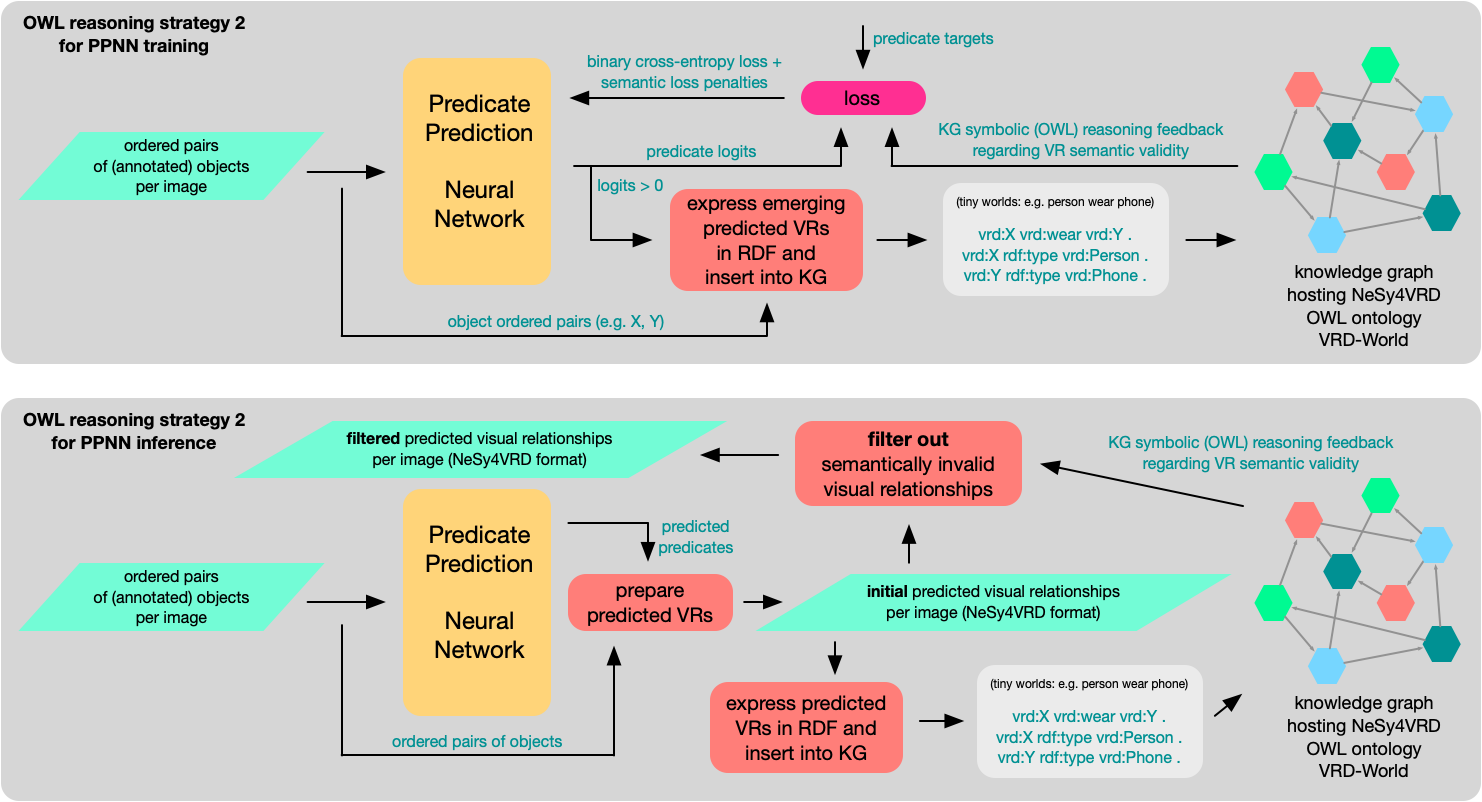
\includegraphics[width=\textwidth]{figs/nesy-system-nnkgs1-training-and-inference-1.png}
  \caption{\footnotesize An illustration of OWL reasoning strategy 2, prediction validation, in action. The top panel shows the setting for PPNN training, the bottom panel for PPNN inference.
  In both settings, an OWL-based knowledge graph hosting OWL ontology VRD-World, acting as a real-time symbolic reasoning binary classifier, validates predictions of visual relationships. During PPNN training, predictions classified as semantically invalid (\eg \texttt{dog drive surfboard}) attract semantic loss penalties, as soft logical constraints. During PPNN inference, predictions classified as semantically invalid are filtered out, as hard logical constraints.}
  \label{fig:nn-kg-s1-setting}
  \Description{An illustration of our OWL reasoning strategy 2: prediction validation. This is a 2-panel plot. Both panels show the predicate detection aspect of our visual relationship detection system, and how that system integrates with our OWL-based knowledge graph. The top panel shows the training setting; the bottom panel shows the inference setting. We insert predicted visual relationships into the KG, and the KG tells us if they are semantically valid or not. We use this feedback to modulate the loss signal used to supervise the learning of the neural network.}
\end{figure}

Figure \ref{fig:nn-kg-s1-setting} summarises OWL reasoning strategy 2, prediction validation, pictorially.
An OWL-based knowledge graph hosting OWL ontology VRD-World acts as a real-time symbolic reasoning binary classifier to validate predictions of visual relationships.
It classifies them as being either semantically valid or invalid.
The hypothesis underlying OWL reasoning strategy 2 is that logical validation of predictions can be leveraged to guide and constrain subsymbolic learning so as to improve predictive performance.
In this case, the primary improvement sought is a lower incidence rate of semantically invalid predicted visual relationships.

During training, if the PPNN's confidence in a certain predicate (for a given ordered pair of objects) rises above a probability of 0.5, the corresponding visual relationship is rendered symbolically as a set of RDF triples and validated by the symbolic reasoning binary classifier.
Assertions of semantically valid visual relationships succeed, and these accumulate within the knowledge graph (along with everything inferred in relation to them).
But assertions of many predictions of visual relationships fail, because they lead to logical inconsistencies in the knowledge graph.
We interpret visual relationships rejected by the knowledge graph---because they lead to logical inconsistencies---as being semantically invalid.

During PPNN training, relationships classified as semantically invalid attract semantic loss penalties.
If we let $c$ (a probability) represent the PPNN's confidence in a hypothetical prediction, and $p$ represent the penalty, then the equation for our semantic loss penalties is $p = - \lambda \log(1 - c),$ where $\lambda$ is a hyperparameter that controls the influence of the penalties.
We set $\lambda = 1$, making our semantic loss penalties rather \emph{soft} logical constraints.
Larger values for $\lambda$ should, in theory, make this constraint harder and more effective.
In Section \ref{sec:summary}, we describe a package of future work for this investigation.
Once a particular predicate (for a given ordered pair of objects) has been identified as semantically invalid, we apply our semantic loss penalty to it \emph{continuously}, each epoch, until training stops, regardless of whether the PPNN's confidence in the predicate falls back below the probability threshold of 0.5.

During PPNN inference (per the bottom panel of Figure \ref{fig:nn-kg-s1-setting}), predicted visual relationships are similarly classified by the symbolic reasoning binary classify.
In this setting, however, a prediction identified as being semantically invalid is \emph{filtered out} of the results submitted for evaluation, in the form of a \emph{hard} logical constraint.
This equates to a logical guarantee that semantically invalid predictions will not emerge from the neurosymbolic system.

We define \emph{treatments} for OWL reasoning strategy 2 (prediction validation) to represent different experiment conditions, and the corresponding trained neurosymbolic systems that are associated with those conditions.
Table \ref{table:invest2-treatments} lists the treatments we discuss in relation to OWL reasoning strategy 2.
For treatment t21, we validate visual relationship predictions during PPNN training only, so that we can evaluate the effectiveness of the associated soft logical constraints in isolation.
For treatment t22, we validate predictions during both PPNN training and inference.
This allows us to evaluate the efficacy of the hard logical constraint of filtering.
Treatment t30 is a special case that combines OWL reasoning strategies 1 and 2.
Here, OWL reasoning strategy 1 (annotation augmentation) is represented by treatment t09 (S\_TEU), which turned out to be the best performing configuration of OWL ontology VRD-World, with respect to recall@N, for OWL reasoning strategy 1.

\begin{table}[t]
  \centering
  \footnotesize
  \begin{threeparttable}
  \caption{\footnotesize Treatment definitions for OWL reasoning strategy 2 (prediction validation).}
  \label{table:invest2-treatments}
  \begin{tabular}{llll}
    \toprule 
     treatment   & treatment  & logical constraints  & logical constraints \\
     name        & key  & applied during PPNN training & applied during PPNN inference \\
    \midrule
    t21 & training only   & soft (semantic loss penalties) &   \\
    t22 & training \& inference   & soft (semantic loss penalties) & hard (filtering-out)  \\
    t30 & t09+t21   & implicit (t09) and soft (t21) &  \\
    \bottomrule 
  \end{tabular}
  \end{threeparttable}
\end{table}

For strategy 2 (prediction validation), we used the free version of OWL-based knowledge graph tool GraphDB~\cite{graphdb} to act as server for our real-time, symbolic reasoning binary classifier.
We configured its integrated OWL reasoning to use its OWL2-RL ruleset, which corresponds to the inference semantics specified for the OWL 2 RL profile.
GraphDB behaved reliably and robustly in the real-time setting of neural network (PPNN) training and inference.
Processing times slowed significantly, especially at first; but as we learned to manage knowledge graph interactions, processing times became more acceptable.
One lesson we learned is to not begin validating predictions immediately, because the random initialisation of a neural network's weights leads to huge numbers of spurious predictions.
We deferred the start of prediction validation to training epoch 3, to give the PPNN a chance to learn its own predictions.
Another lesson we learned is to look for opportunities to eliminate redundant interactions with the knowledge graph, in order that symbolic reasoning is used as efficiently and sparingly as feasible.
In our case, every visual relationship is an instance of a \emph{type}, and once the \emph{type} is classified as valid or invalid (triggered by an encounter with a first instance), so are all further instances.
We devised an efficient cache for saving the symbolic classifier's visual relationship (type) decisions, and looked to the cache first, before going to the classifier (the knowledge graph).
Further operational details relating to the handling of knowledge graph interactions, and the management of the knowledge graph itself, can be found in \citet{HerronThesis2025}.

Lastly, since the objective of OWL reasoning strategy 2 (prediction validation) is to reduce the incidence of semantically invalid predictions (which have no chance of being hits), we verified that every visual relationship annotated for the NeSy4VRD training set and test set images is semantically valid (according to OWL ontology VRD-World).
To accomplish this task, we used our visual relationship symbolic reasoning binary classifier to validate each one---a demonstration of the OWL classifier contributing during analysis, as well as neural network training and inference.




\subsection{Metrics}
\label{sec:metrics}

Here we discuss many of the metrics we used for evaluating the effects of our OWL reasoning strategies on the subsymbolic learning of our PPNN (and, by extension, on the visual relationship detection system).
We begin by explaining how predicted visual relationships are matched with target (annotated) ones, so that the concept of a \emph{hit} is clear.
We discuss our use of recall@N, and provide some background in relation to this decision, including the challenges that exist with respect to using precision-related metrics.
We describe our use of mAP@N (mean average precision), and explain why we use it despite these challenges. 
We discuss how we measure precision manually (on a small random sample of test set images) to get a truer impression of the impact of OWL reasoning upon precision than mAP@N is able to provide.
We also introduce the notions of a `false false positive', and a corresponding metric we call the  `false false positive rate' (FFPrate).
These notions help us to probe more deeply into the precision of the PPNN, and provide another perspective from which to evaluate the effects of OWL reasoning.

\subsubsection{Matching and hits}
In the discussion of predicate detection, in Section \ref{sec:baseline-system}, we explained that our PPNN predicts predicates for corresponding ordered pairs of objects ($X$ and $Y$, say).
These three elements, \texttt{($X$ predicate $Y$)}, represent a visual relationship, where each object is represented by a bounding box and an object class label.
Thus, for evaluation purposes, a visual relationship (predicted or annotated) has five elements.
If the five elements of a predicted visual relationship (for a given image) match the corresponding five elements of an annotated (target) visual relationship (for the same image), we count a \emph{hit} (a true positive).
The requirement for a match between two bounding boxes is that their IoU (intersection over union) be 0.5 or more.
But since the research we discuss pertains to the predicate detection subtask of visual relationship detection (where we use annotated objects in place of detected ones), if two objects match, they match exactly, with IoU 1.

\subsubsection{recall@N}
Beginning with the paper that first introduced the VRD dataset \cite{lu2016visual}, researchers using it have focused virtually exclusively on measuring recall@50 and recall@100 to compare the performance of their respective visual relationship detection systems.
The reason for the focus on recall is that the images of the VRD dataset (and, similarly, of our NeSy4VRD dataset) are \emph{not annotated exhaustively}, either in terms of objects or relationships.
Exhaustive manual annotation is infeasible.
The consequence is that counts of false positive visual relationships are exaggerated, because perfectly good predictions, of things that simply were not annotated (but might well have been), are treated as false positives.
This leads to precision-related metric scores that can be grossly pessimistic and misleading.

We continue the convention of measuring recall@50 and recall@100, and for the same reasons, but we expand this set of metrics to include recall@25 and recall@999 to help us discern effects of OWL reasoning on the subsymbolic learning of our PPNN---which is our prime objective (not visual relationship detection for its own sake).
The recall@N metric that we use is more precisely described as `mean per image recall@N'.
That is, we calculate recall@N scores for each test set image, and then take the average.
The recall@N metric used by \citet{lu2016visual} (and perhaps others) is different---they use a global (or macro) measure: the ratio of total hits @N (across all images) to total annotated (ground-truth) relationships (across all images).
We found that both recall@N metrics (global, and mean per image) delivered similar scores and responded to the stimulus of OWL reasoning in similar ways.
We preferred `mean per image' recall@N in order to be consistent with our other metrics, such as volume of predictions and mAP@N.

For OWL reasoning strategy 1 (annotation augmentation), recall@N is a primary metric.
For strategy 2 (prediction validation), it is secondary, since the goal there is to reduce the incidence of semantically invalid predictions.
We also calculate standard recall in relation to OWL reasoning strategy 2, for a small random sample of test set images whose predicted visual relationships are inspected manually.

\subsubsection{mAP@N}
Despite the challenges associated with precision-related metrics just described, we opted to measure mAP@N (mean average precision), and for the same values of $N \in \{25, 50, 100, 999\}$, just as for recall@N.
The justification is that, while the mAP@N scores will not be meaningful in absolute terms, the changes in the mAP@N treatment scores, relative to baseline, and relative to one another, can still reveal useful insights into the effects of OWL reasoning.
First, we compute average precision (AP) for each test set image, using
\begin{displaymath}
  AP = \sum_{k=1}^n p(k) \Delta r(k) = \sum_{k=1}^n p(k) \Big(r(k) - r(k-1)\Big),
\end{displaymath}
where $k$ is the rank in a set of predicted visual relationships sorted in descending order by confidence, $n$ is the number of predicted visual relationships, $p(k)$ is the precision at cut-off $k$, and $\Delta r(k)$ is the change in recall from items $k-1$ to $k$.
Since $r(0)$ is not defined, we set $r(0) = 0$.
Then we average the per-image AP scores to get mAP@N, using
\begin{displaymath}
  mAP = \frac{\sum_{t=1}^T AP(t)}{T},
\end{displaymath}
where $T$ is the number of NeSy4VRD test set images.

\subsubsection{Precision, adjusted precision, and `false false positve rate'}
To get truer estimates of precision (in absolute terms) than mAP@N could provide, we measured precision manually, via visual inspection.
We randomly selected a small subset (25) of the test set images, from amongst those having more than 8 but less than 25 predicted visual relationships.
This latter condition helped keep this manual exercise tractable, and it had the added benefit that the scores calculated correspond simultaneously to all values of $N \in \{25, 50, 100, 999\}$ for a hypothetical precision@N metric.
We displayed each predicted visual relationship, individually, against its associated image, and simultaneously observed whether or not it had been marked as a \emph{hit} or not.
It was soon clear that the majority of predictions not marked as hits were, in fact, perfectly good predictions of visual relationships that might well have been annotated, but simply had not been.
So each predicted visual relationship not marked as a hit (\ie each ostensible false positive, or FP) was further classified as being either a true false positive (TFP) or a false false positive (FFP), giving, for each image, $FP = TFP + FFP$, and where: 
\begin{itemize}
  \item TFP = true false positive (\ie definitely a bad prediction)
  \item FFP = false false positive (\ie either definitely good or a borderline case).
\end{itemize}

This factorisation (or classification) of FPs permitted us to compute two measures of precision: the standard one, and an adjusted one that excludes the FFPs.
Thus, standard precision (per image) was measured using
\begin{displaymath}
  precision = \frac{TP}{TP + FP} = \frac{TP}{TP + (TFP + FFP)}, 
\end{displaymath}
and \emph{adjusted} precision (per image) was measured using
\begin{displaymath}
  precision_{adj} = \frac{TP}{TP + TFP}.
\end{displaymath}

The classification of the FPs also permitted us to devise a further metric that we call the `false false positive rate', or FFP rate, for short.
This measures the proportion of FPs (the non-hits) that, upon visual inspection, were deemed to be good predictions of visual relationships.
The FFP rate is defined as
\begin{displaymath}
  FFPrate = \frac{FFP}{FP} = \frac{FFP}{TFP + FFP}.
\end{displaymath}

\subsubsection{Learning speed}
For OWL reasoning strategy 1 (annotation augmentation), we evaluate the learning speed of the PPNN, measured in training epochs.
In Section \ref{sec:baseline-system}, we explained that every epoch we save a model checkpoint.
The first model checkpoint (\ie the lowest training epoch) to deliver the maximum observed recall@N score, for $N \in \{25, 50, 100, 999\}$, is selected for evaluation.
We treat the epoch numbers of these ($topN$-specific) `earliest best performing models' as measures of PPNN (subsymbolic) learning speed.

\subsubsection{Incidence rate of semantically invalid predictions}
The primary metric for evaluating OWL reasoning strategy 2 (prediction validation) is the incidence rate of semantically invalid predicted visual relationships.
As explained in Section \ref{sec:kg4pval-methods}, strategy 2 was conceived to reduce this rate.
We measure this incidence rate by counting the individual instances of predicted visual relationships that are found to be semantically invalid.
To get these counts for our baseline deep learning system, for example, we used our symbolic reasoning binary classifier (our OWL-based knowledge graph hosting OWL ontology VRD-World) to post-process (post-classify) its predictions.
Our symbolic reasoning binary classifier thus played a key role not just in neural network (PPNN) training and inference, but in the analysis of results as well. 

\subsubsection{Volume of predictions per image}
We also examine the mean number of predicted visual relationships per image.
This metric yields findings that are interesting in themselves, and that help us better understand the recall@N and mAP@N scores that we observe.

\subsubsection{Symmetric pairs and inverse pairs}
Finally, for OWL reasoning strategy 1 (annotation augmentation), we also do a deep dive into the effects of two particular subcategories of OWL link inference semantics: symmetry and inverses.
We devised several metrics to help us probe the extent to which \emph{symmetry} inferences being activated leads to the PPNN learning to better predict visual relationships in symmetric pairs.
We measure things such as \textit{(a)} the mean number of predicted visual relationships (VRs) where the predicate is a symmetric property (per VRD-World), \textit{(b)} the mean number of predicted VRs that belong to a symmetric pair (regardless of topN rank), \textit{(c)} the mean number of predicted VRs that belong to a symmetric pair, where the pair is within the same topN rank of predictions, and \textit{(d)} the mean number of hits where the predicate is symmetric.
We also devised counterpart metrics to help us probe the extent to which \emph{inverse} inferences being activated leads to the PPNN learning to better predict visual relationships in inverse pairs.



% = = = = = = = = = = = = = = = = = = = = = = = = = = = = = = = = = =



\section{Evaluation}
\label{sec:evaluation}

In this section we report and discuss our research findings.
First we discuss findings that relate to OWL reasoning strategy 1 (annotation augmentation).
The figures, tables, and discussions refer heavily to the various \emph{treatments} that we defined for this strategy earlier, detailed in Table \ref{table:invest1-treatments}. 
Remember that OWL reasoning strategy 1 treatments represent configurations of OWL link inference semantics (\ie different rules activated or deactivated), and the corresponding systems that emerge from having trained on image scene graphs that were logically augmented using these different configurations.

Then we discuss findings that relate to OWL reasoning strategy 2 (prediction validation).
Recall that strategy 2 also has \emph{treatments}, defined in Table \ref{table:invest2-treatments}, but whose nature is quite different to that of the strategy 1 treatments.
For strategy 2, there are just two main treatments: one that uses predication validation during PPNN training only, and one that uses it during PPNN training and inference.
As readers will see, as we discuss the effect of OWL reasoning strategy 2 on reducing the incidence of predictions of semantically invalid visual relationships, we also examine the effects of annotation augmentation towards this same goal (using one of the OWL reasoning strategy 1 treatments).
We also refer to a treatment that combines strategies 1 and 2, so we can examine how the two strategies co-operate in reducing semantically invalid predictions.

For each experiment scenario, whether for the baseline deep learning system or for a neurosymbolic treatment system, we trained and evaluated four system instances for the scenario.
Thus, the findings that we present have underlying sample sizes of four.
We make frequent use of boxplots, where the boxes represent the distributions of four sample points.
Most of the time, these boxes are reassuringly small, indicating the presence of little variation within the small sample sizes, and providing evidence of the efficacy of our approach to model selection (as described in Section \ref{sec:baseline-system}).

\subsection{Effects of OWL reasoning strategy 1 - annotation augmentation}

\subsubsection{On the volume of predictions}

Figure \ref{fig:nnkgs0-owl-re-on-npvrs-per-image} shows the effects of using OWL reasoning strategy 1 (annotation augmentation) on the mean number of visual relationships predicted per image.
As explained earlier, in Section \ref{sec:methods-strategy-1}, each \emph{treatment} (t01, t02, etc.) represents a different configuration of OWL link inference semantics having been activated within OWL ontology VRD-World for the logical expansion of the training image scene graphs used to supervise PPNN training.
It is clear that many of the neurosymbolic treatment systems generate far greater volumes of predictions per image than the baseline deep learning visual relationship detection system, which does not benefit from leveraging OWL reasoning. 

\begin{figure}
\center
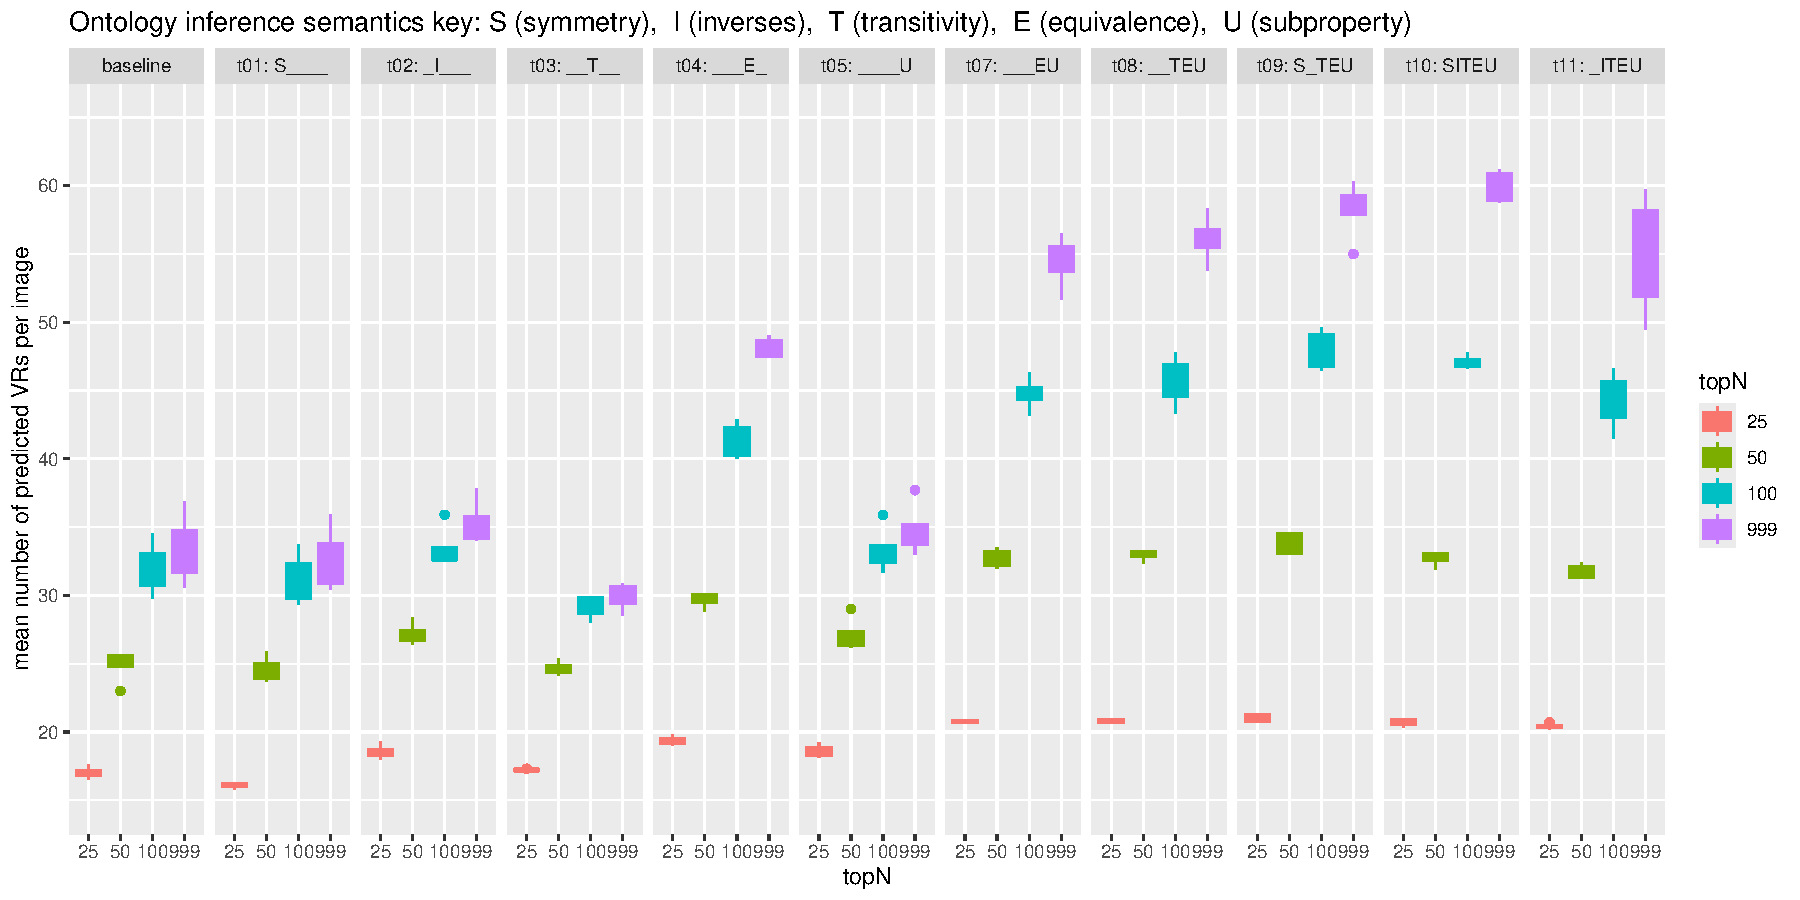
\includegraphics[width=1.0\textwidth]{figs/plot_v8_p18b_RStudioExport_12x6.pdf}
\caption{\footnotesize The effects of OWL reasoning strategy 1 (annotation augmentation) on the mean number of visual relationships predicted per NeSy4VRD test set image. Different mixtures of OWL link inference semantics within OWL ontology VRD-World lead to differently augmented training image scene graphs, and these induce different volumes of predicted visual relationships---many of which far exceed the volumes generated by a baseline system, where deep (subsymbolic) learning does not benefit from leveraging OWL reasoning.}
\label{fig:nnkgs0-owl-re-on-npvrs-per-image}
\Description{A boxplot showing the effects of OWL reasoning strategy 1 (annotation augmenation) on the mean number of visual relationships predicted for the NeSy4VRD test set images. The figure is faceted horizontally. Each facet shows the results for one trained system: the baseline deep learning system, and several neurosymbolic treatment systems (which employed annotation augmentation in a particular way). For each system/facet (baseline or treatment), four boxes (distributions of scores) are plotted, one for each of the topN values of 25, 50, 100 and 999.}
\end{figure}

The activation or deactivation of different OWL link inferences is the only variable that changes across the neurosymbolic treatment systems, so it is the OWL inferences alone that are \emph{causally determining} the different prediction volume outcomes seen in Figure \ref{fig:nnkgs0-owl-re-on-npvrs-per-image}.
The different logical expansions of the training image scene graphs guide and constrain the (subsymbolic) learning of the PPNN so as to induce it to predict dramatically different volumes of visual relationships.

Another observation is the striking difference in prediction volume outcomes that arise when the subcategories of OWL link inference semantics are used in combination with one another (as in treatments t07 through t11), as opposed to individually (as in treatments t01 through t05).
When used individually, the corresponding logical expansions of the training image scene graphs have little impact on prediction volumes, except for treatment t04 (\_\_\_E\_), which is a notable exception.
But when used in combination with one another, Figure \ref{fig:nnkgs0-owl-re-on-npvrs-per-image} provides evidence of interesting \emph{interactions} between the subcategories of OWL link inference semantics, many of which appear to be \emph{co-operative} or \emph{mutually reinforcing}.
For example, the ontology subproperty relationships of treatment t05 (\_\_\_\_U), by themselves, have little impact on system prediction volumes.
But when subproperty relationships (U) are used in combination with property equivalence relationships (E), as in treatment t07 (\_\_\_EU), the two subcategories of link inference semantics appear to collaborate with one another constructively, to induce even greater numbers of predictions from the subsymbolic learning of the PPNN. 
Similarly, the symmetry of treatment t01 (S\_\_\_\_), by itself, has no impact.
But when combined with treatment t08 (\_\_TEU), to give treatment t09 (S\_TEU), symmetry helps to boost prediction volumes relative to those of t08.

\subsubsection{On recall@N}

\begin{figure}[t]
\center
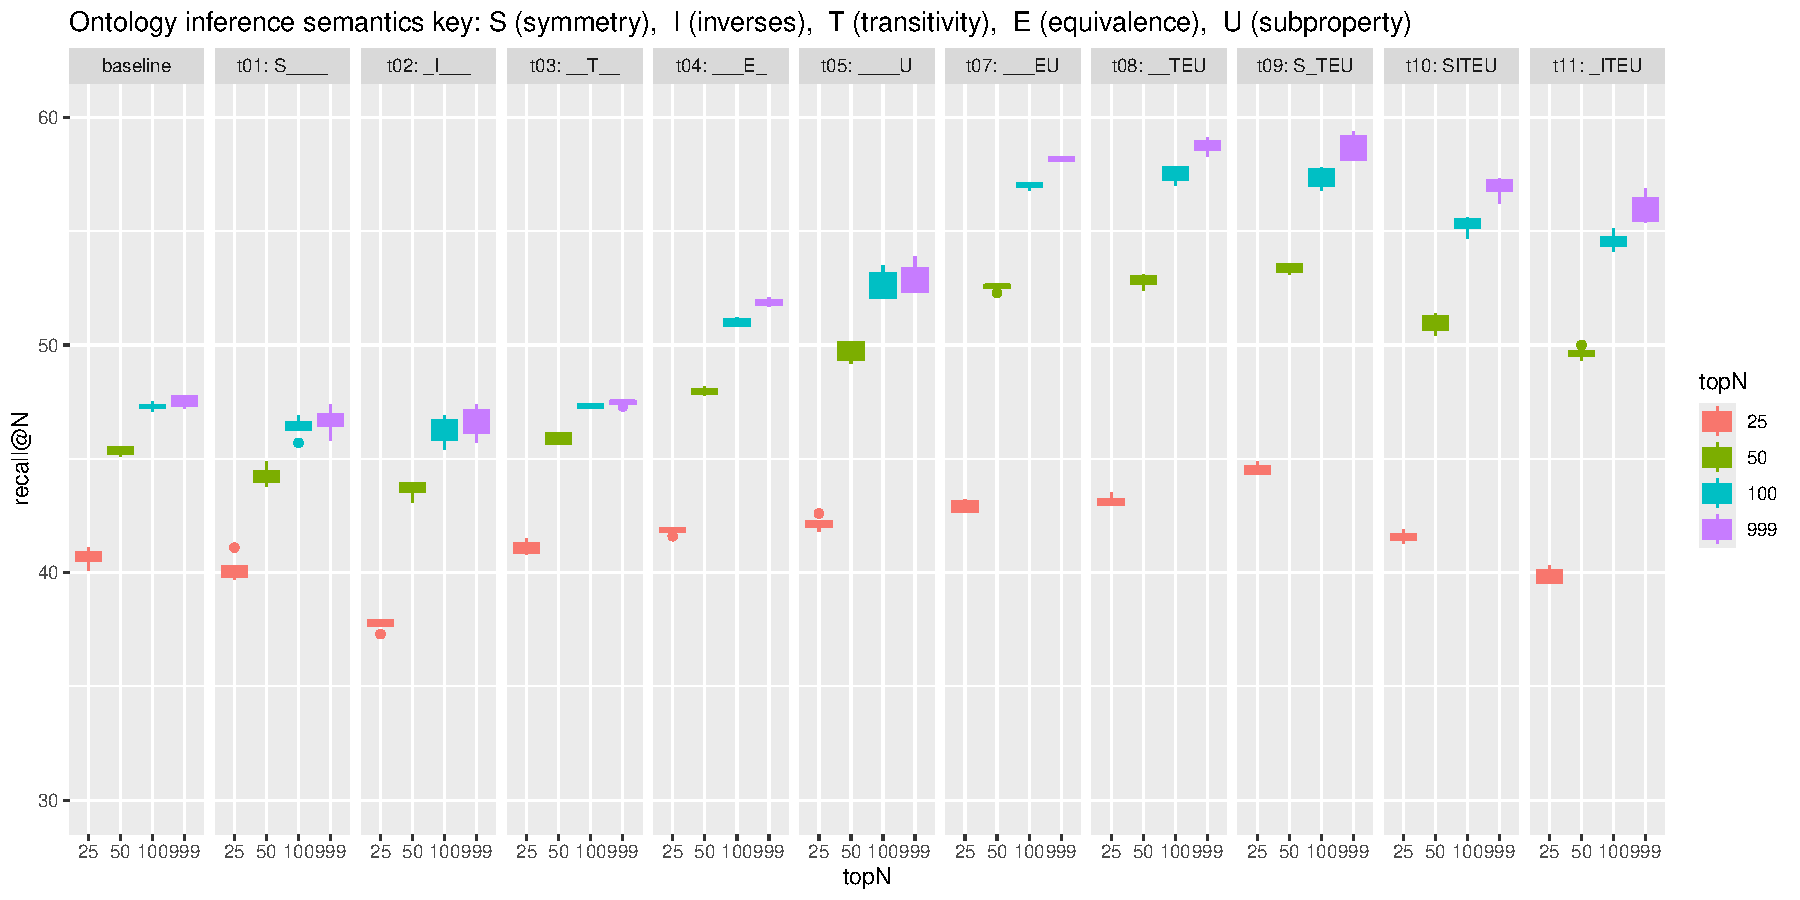
\includegraphics[width=1.0\textwidth]{figs/plot_v8_p15b-owl-re-on-recall-base_12x6.pdf}
\caption{\footnotesize The effects of OWL reasoning strategy 1 (annotation augmentation) on recall@N. Different treatments (combinations of OWL link inference semantics in OWL ontology VRD-World) used to logically expand training image scene graphs permit many of the corresponding neurosymbolic treatment systems to outperform a baseline system, where deep (subsymbolic) learning does not benefit from leveraging OWL reasoning.}
\label{fig:nnkgs0-owl-re-on-recall-baseline}
\Description{A boxplot showing the effects of OWL reasoning strategy 1 (annotation augmenation) on recall@N. The figure is faceted horizontally. Each facet shows the results for one trained system: the baseline deep learning system, and several neurosymbolic treatment systems (which employed annotation augmentation in a particular way). For each system/facet (baseline or treatment), four boxes (distributions of scores) are plotted, one for each of the topN values of 25, 50, 100 and 999.}
\end{figure}

Figure \ref{fig:nnkgs0-owl-re-on-recall-baseline} shows the effects of using OWL reasoning strategy 1 (annotation augmentation) on recall@N scores, for the same treatments as in Figure \ref{fig:nnkgs0-owl-re-on-npvrs-per-image}.
It is clear that many of the neurosymbolic treatment systems (which leverage symbolic OWL reasoning) strongly outperform the baseline deep learning system.
This is especially the case for treatment systems t07 through t11, where combinations of OWL link inference semantics in ontology VRD-World are used to logically expand training image scene graphs.
But treatments t04 (property equivalence semantics, alone) and t05 (subproperty semantics, alone) also outperform the baseline, albeit to a lesser extent.

The prediction volume scores in Figure \ref{fig:nnkgs0-owl-re-on-npvrs-per-image} help to explain many of the corresponding treatment recall@N scores.
Higher recall@N tends to be associated with higher prediction volumes, which makes sense.
But there are exceptions to this general rule.
First, recall@N for treatment t05 (\_\_\_\_U) increases strongly relative to baseline, but without any corresponding increase in prediction volumes relative to baseline.
This suggests that precision has improved.
Second, recall@N for treatment t10 (SITEU), which has all five subcategories of OWL link inference activated simultaneously, falls relative to that for treatment t09 (S\_TEU), yet t10 generates as many predictions as t09.
This suggests a decrease in precision.

Figure \ref{fig:nnkgs0-owl-re-on-recall-baseline} also reveals further evidence of \emph{interactions} between the subcategories of OWL link inference semantics that are used to logically expand the training image scene graphs.
First, consider treatment t07 (\_\_\_EU), which combines the inference semantics of treatments t04 and t05.
Here we see co-operative interaction that appears to be virtually \emph{additive}.
For recall@100, say, the uplift from baseline for t04 is about 4 percentage points (47\% to 51\%); the uplift from baseline for t05 is about 5.5 percentage points; and the uplift from baseline for t07 is about 10 points.
Second, the contributions to recall@N of the inference semantics of symmetry changes depending on whether it is used alone or in combinations.
By itself, its contribution is negative: recall@N for treatment t01 falls slightly (relative to baseline).
But in combination treatments, the contributions of symmetry are positive.
Adding it to treatment t08 (\_\_TEU), giving t09 (S\_TEU), increases recall@25 and recall@50; and removing it from treatment t10 (SITEU), giving t11 (\_ITEU), leads to recall@N falling for all values of $N$.
In contrast to symmetry, the contributions to recall@N of the inference semantics of inverses do not change: they are consistently negative.
Whether alone (as in treatment t02), or when added to treatment t09 (S\_TEU), giving treatment t10 (SITEU), the semantics of inverse relationships is associated with reductions in recall@N.

Note that the recall@N scores in Figure \ref{fig:nnkgs0-owl-re-on-recall-baseline} pertain to treatment systems that were \emph{trained} on \emph{logically augmented} training image scene graphs but \emph{evaluated} against \emph{baseline} (\ie non-augmented) test set image scene graphs.
This setting gives OWL reasoning its best opportunity to show evidence of its effects on subsymbolic learning.
\citet{HerronThesis2025} also reports recall@N results generated by counterpart treatment systems that were trained on \emph{logically augmented} training image scene graphs and evaluated against \emph{correspondingly logically augmented} test set image scene graphs.
These latter recall@N scores are surprisingly similar to the former (Figure \ref{fig:nnkgs0-owl-re-on-npvrs-per-image}), despite the fact that the expanded test set scene graphs (expanded targets) make the visual relationship detection task harder---with many more targets to be hit. 
This is evidence of how well the logical regularities reflected in the expanded training image scene graphs are captured by the subsymbolic learning of the PPNN.

\subsubsection{On mAP@N and precision}

\begin{figure}[t]
\center
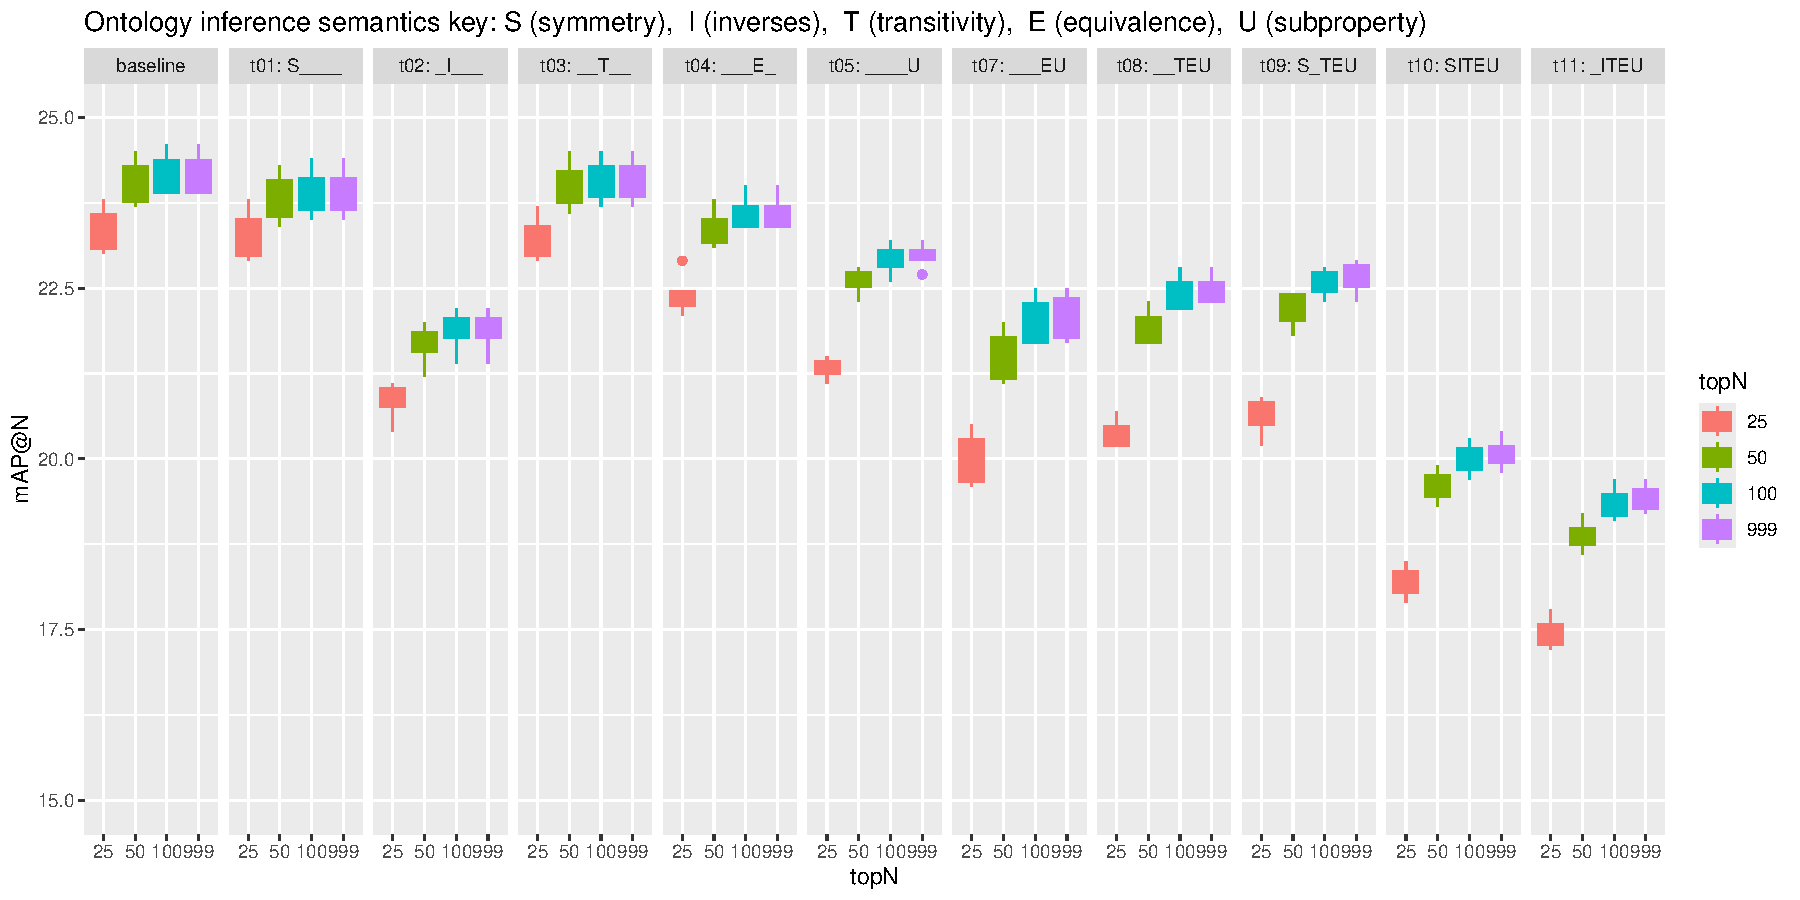
\includegraphics[width=1.0\textwidth]{figs/plot_v8_p17b_RStudioExport_12x6.pdf}
\caption{\footnotesize The effects of OWL reasoning strategy 1 (annotation augmentation) on mAP@N. Different neurosymbolic treatments (combinations of OWL link inference semantics in OWL ontology VRD-World used to logically expand training image scene graphs) deliver mAP@N scores lower than a baseline deep learning system, to varying degrees. The salient observation, however, is how well mAP@N \emph{endures}, given the corresponding, but far larger, relative increases in treatment prediction volumes induced by OWL reasoning strategy 1 (shown elsewhere).}
\label{fig:nnkgs0-owl-re-on-mAP}
\Description{A boxplot showing the effects of OWL reasoning strategy 1 (annotation augmenation) on mAP@N. The figure is faceted horizontally. Each facet shows the results for one trained system: the baseline deep learning system, and several neurosymbolic treatment systems (which employed annotation augmentation in a particular way). For each system/facet (baseline or treatment), four boxes (distributions of scores) are plotted, one for each of the topN values of 25, 50, 100 and 999.}
\end{figure}

Figure \ref{fig:nnkgs0-owl-re-on-mAP} shows the effects of using OWL reasoning strategy 1 (annotation augmentation) on mAP@N scores, for the same treatments as in Figures \ref{fig:nnkgs0-owl-re-on-npvrs-per-image} and \ref{fig:nnkgs0-owl-re-on-recall-baseline}.
Most of the neurosymbolic treatment systems underperform the baseline deep learning system with respect to mAP@N.
The decreases in the mAP@N scores are, however, well explained by corresponding increases (relative to baseline) in treatment system prediction volumes, as seen earlier, in Figure \ref{fig:nnkgs0-owl-re-on-npvrs-per-image}.
Once the increases in underlying prediction volumes are taken into account, the scale of the reductions in mAP@N relative to baseline look remarkably \emph{small}.
For example, consider neurosymbolic treatment t09 (S\_TEU) relative to baseline.
Figure \ref{fig:nnkgs0-owl-re-on-npvrs-per-image} shows that the baseline deep learning system generates (for topN=999) about 33 visual relationship predictions per image, on average, whereas treatment t09 generates about 59---a relative increase in prediction volumes of 79\%.
Figure \ref{fig:nnkgs0-owl-re-on-mAP} shows that the baseline system's mAP@999 score is about 24\%, whereas the score for treatment t09 falls to 22.5\%---a relative decrease of just 6\%.
Thus, the key observation is not that mAP@N falls for the neurosymbolic treatment systems, but how well it \emph{endures}, given the large increases in underlying prediction volumes induced by OWL reasoning strategy 1.

Another essential observation is that the \emph{absolute values} of the mAP@N scores in Figure~\ref{fig:nnkgs0-owl-re-on-mAP} are grossly pessimistic and misleading.
Metrics like mAP (mean average precision) assume exhaustive annotation, which enables false positives to be identified reliably.
But, as explained earlier, in Section \ref{sec:metrics}, the images of NeSy4VRD are \emph{not} annotated exhaustively, so false positives cannot be identified reliably, and they get over-counted as a consequence.
That is, many predicted visual relationships that fail to match any annotated (target) visual relationship are perfectly good predictions of relationships that might have been annotated but were not.
The mAP@N metric cannot distinguish these \emph{false} false positives from the \emph{true} false positives.
Hence, when considering Figure \ref{fig:nnkgs0-owl-re-on-mAP}, the useful information lies in the \emph{relative changes} in the mAP@N scores, not their absolute values.

For example, Figure \ref{fig:nnkgs0-owl-re-on-mAP} gives helpful insight into the contributions of the OWL link inference semantics of inverses.
Figure \ref{fig:nnkgs0-owl-re-on-mAP} shows that, for treatment t02 (\_I\_\_\_), mAP@N scores fall distinctively relative to baseline, yet Figure \ref{fig:nnkgs0-owl-re-on-npvrs-per-image} shows no corresponding relative increase in prediction volumes to help explain this fall.
We see a similarly distinctive relative fall in mAP@N between treatments t09 (S\_TEU) and t10 (SITEU), yet Figure \ref{fig:nnkgs0-owl-re-on-npvrs-per-image} shows that these treatments generate similar volumes of predictions.
This evidence clearly associates the inference semantics of inverses with lower precision, as measured by mAP@N, at least.

\begin{table}[t]
  \centering
  \footnotesize
  \begin{threeparttable}
  \caption{\footnotesize The effects of OWL reasoning strategy 1 (annotation augmentation) on precision, as  measured manually via visual inspection of individual predicted visual relationships (VRs), for a small random sample of test set images. The adjusted precision scores exclude \emph{false} false positives (FFPs) from consideration. The FFP rate gives the proportion of false positives deemed to be good predictions of visual relationships not annotated. Standard recall is hits per image over ground-truth annotations per image.}
  \label{table:manual-precision-scores}
  \begin{tabular}{lrrrrrr}
    \toprule
            & mean       & mean       & mean       & mean   & \% change & mean \\
     model  & precision  & precision  & FFP  & predicted VRs & predicted VRs & recall \\
            & (standard)  & (adjusted) & rate  & per image & per image & (standard) \\
            & (\%)   &  (\%)  & (\%) & (count) & (\% chg) & (\%) \\
    \midrule
    baseline & 30.2  & \textbf{71.7}  & 78.1 & 11.9 &  & 47.4 \\
    t09 (S\_TEU) & 21.2  & 65.9  & \textbf{82.8} & \textbf{18.4} & 53.8 & \textbf{50.9} \\
    \bottomrule 
  \end{tabular}
  \end{threeparttable}
\end{table}

To get a better sense of the precision delivered by our baseline deep learning and our neurosymbolic treatment systems in \emph{absolute} terms, we measured precision manually during visual inspection of the individual visual relationships predicted for a random sample of 25 test set images.
Table \ref{table:manual-precision-scores} reports the findings of this exercise, for the baseline deep learning system and the neurosymbolic treatment system t09 (S\_TEU)---the one that delivers maximal recall@N, per Figure \ref{fig:nnkgs0-owl-re-on-recall-baseline}. 
The standard precision scores are roughly in line with the mAP@N scores in Figure \ref{fig:nnkgs0-owl-re-on-mAP} and, like them, are grossly pessimistic and misleading.
As explained earlier, in Section \ref{sec:metrics}, our \emph{adjusted} precision metric excludes \emph{false} false positives (FFPs) (\ie good predictions of visual relationships not annotated).
So the scores for `adjusted precision' are the ones that provide truer estimates of precision in absolute terms.
We see that adjusted precision for treament t09 falls relative to baseline, from a respectable 71.7\% to 65.9\%---a relative decrease of 8\%.
But given the relative increase in underlying prediction volumes of 79\% (mentioned earlier), and given the relative increase of 53.8\% reported in Table \ref{table:manual-precision-scores} for the random sample of 25 images, this 8\% relative fall in adjusted precision is remarkably small. 

Also explained earlier, in Section \ref{sec:metrics}, the FFP rate reported in Table \ref{table:manual-precision-scores} gives the proportion of predicted visual relationships that fail to match an annotated (ground-truth) target that are, upon visual inspection, deemed to be good predictions of visual relationships that were simply not annotated.
With respect to this metric, we see that the neurosymbolic treatment t09 (S\_TEU) system outperforms the baseline deep learning system, lifting the FFP rate from 78.1\% to 82.8\%.

The increase in (standard) recall relative to baseline reported in Table \ref{table:manual-precision-scores} for treatment t09, from 47.4 to 50.9, is consistent with the moderate increases in recall@25 seen earlier, in Figure \ref{fig:nnkgs0-owl-re-on-recall-baseline}.
Recall@25 is the only comparable metric in Figure \ref{fig:nnkgs0-owl-re-on-recall-baseline} because, as explained earlier, in Section \ref{sec:metrics}, the random sample of 25 images being analysed is drawn from the set of test set images for which the baseline system generated between 8 and 25 predictions, in order to keep the manual analysis tractable.
Treatment t09 generated moderately more predictions per image---an average of 18.4 versus 11.9 for baseline.
This is a healthy increase of 50\%, but the volume of predictions still corresponds to a recall@25 metric only.
For treatment t09, Figure \ref{fig:nnkgs0-owl-re-on-recall-baseline} shows recall@25 increasing (relative to baseline) from 41 to 44.
So the scale of the score increases for the two measures of recall (standard recall, and recall@25), relative to baseline, are consistent.
The discrepancies in the absolute values are explained by the small size of our random sample.

\subsubsection{On learning speed}

\begin{figure}
\center
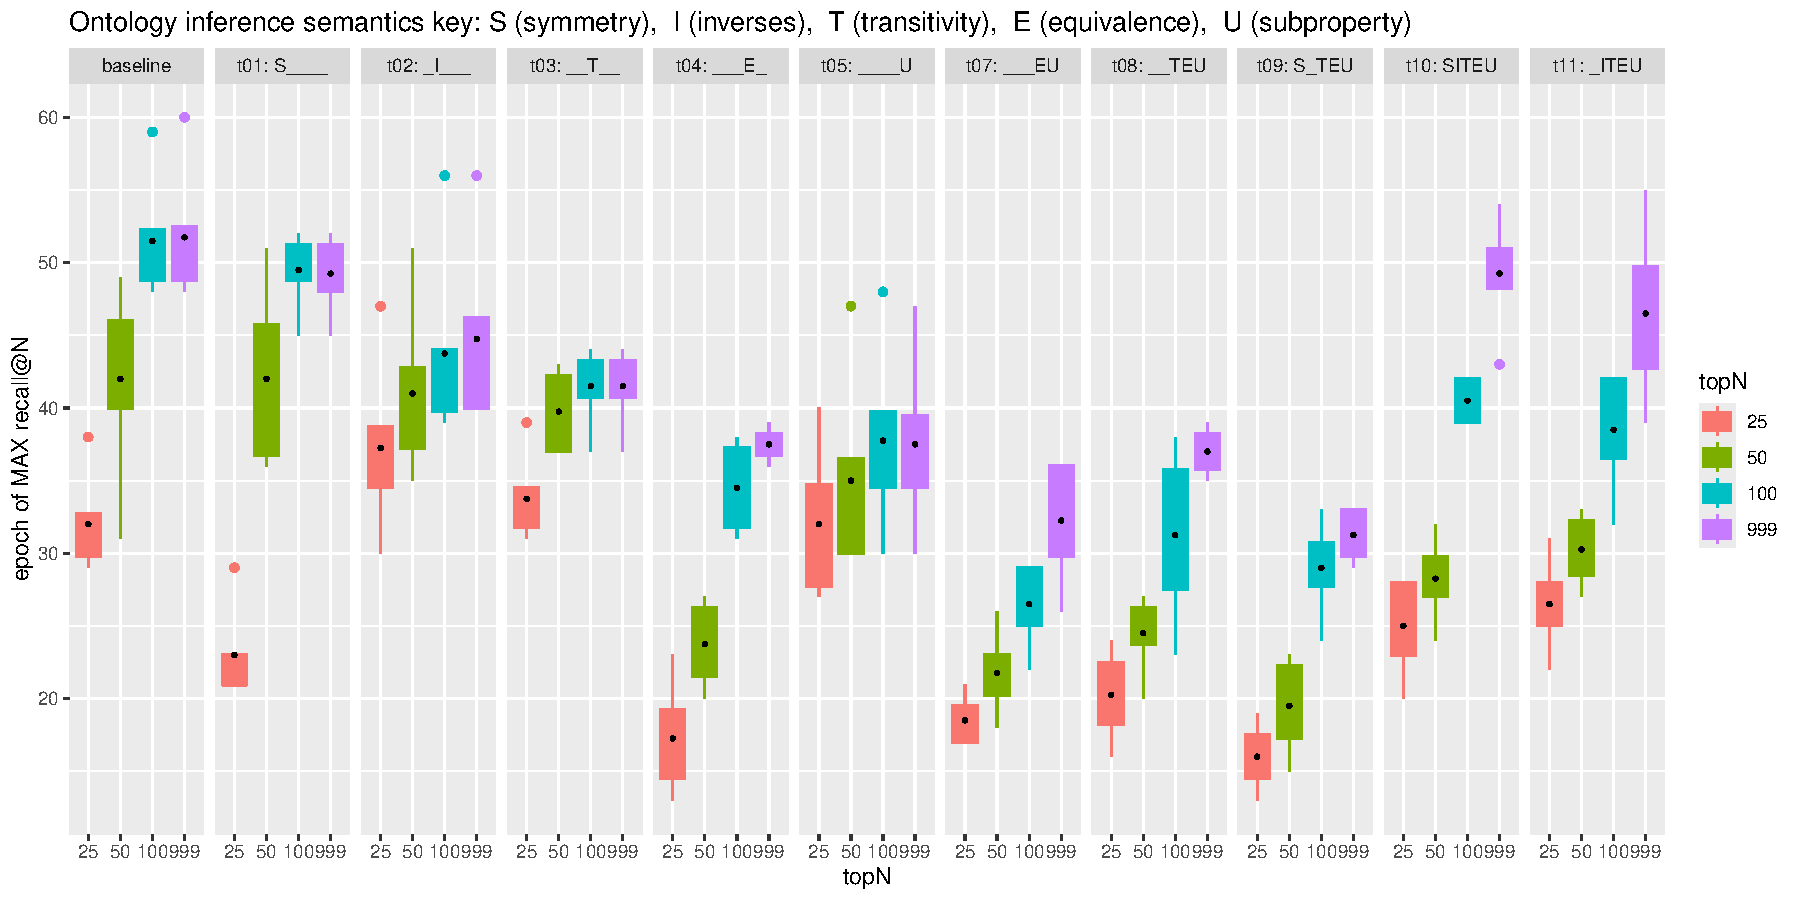
\includegraphics[width=\textwidth]{figs/plot_v8_p7b3-owl-re-on-speed-of-learning_12x6.pdf}
\caption{\footnotesize The effects of OWL reasoning strategy 1 (annotation augmentation) on the speed of subsymbolic learning of a predicate prediction neural network (PPNN). Learning speed is measured in training epochs. The black dots indicate the means of the distributions of epoch numbers. The different neurosymbolic treatment systems (that use combinations of OWL link inference semantics in OWL ontology VRD-World to logically expand training image scene graphs) tend to learn faster than a baseline deep learning system, reaching their maximum observed recall@N scores with model checkpoints having lower epoch numbers.}
\label{fig:nnkgs0-owl-re-on-speed-of-learning}
\Description{A boxplot showing the effects of OWL reasoning strategy 1 (annotation augmenation) on the learning speed of our predicate detector. Learning speed is measured in training epochs. Fewer is faster. The figure is faceted horizontally. Each facet shows the results for one trained system: the baseline deep learning system, and several neurosymbolic treatment systems (which employed annotation augmentation in a particular way). For each system/facet (baseline or treatment), four boxes (distributions of scores) are plotted, one for each of the topN values of 25, 50, 100 and 999.}
\end{figure}

Figure \ref{fig:nnkgs0-owl-re-on-speed-of-learning} shows the effects of using OWL reasoning strategy 1 (annotation augmentation) on the speed with which our (subsymbolic) PPNN model learns.
As explained earlier, in Section \ref{sec:metrics}, we measure learning speed using the epoch numbers of the `earliest best performing models', with respect to recall@N, as measures of PPNN (subsymbolic) learning speed.
We see that logical expansion of the training image scene graphs is strongly associated with lower epoch numbers.
In other words, the neurosymbolic treatment systems tend to learn \emph{faster} than the baseline deep learning system.

Part of an explanation for the faster learning evidenced in Figure \ref{fig:nnkgs0-owl-re-on-speed-of-learning} is that the logical expansions of the training image scene graphs lead to richer mini-batch loss signals that convey more and/or better supervisory information, so fewer training epochs are needed for the model to consume all available supervisory value and reach maximal recall@N.
But this narrative does not explain everything.
For example, consider the contributions of the OWL inference semantics of inverses.
When it participates in combinations, as in treatments t10 (SITEU) and t11 (\_ITEU), the speed of subsymbolic learning slows (\ie the epoch numbers increase) markedly.
It is as if the inference semantics of inverses brings confusion to the subsymbolic learning process rather than clarity.

\subsubsection{On predicting visual relationships in symmetric pairs}

Table \ref{table:symmetric-pairs-in-pred-vrs} shows the effects of OWL reasoning strategy 1 (annotation augmentation) on the prediction of visual relationships in symmetric pairs.
The analysis covers the baseline deep learning system and several neurosymbolic treatment systems in which the inference semantics of symmetry is activated when the logical expansion of the training image scene graphs is performed. 
The basic hypothesis is that logically expanded training image scene graphs---that reliably contain visual relationships having symmetric predicates in symmetric pairs---should help the subsymbolic PPNN learn to predict visual relationships in symmetric pairs.
In other words, the subsymbolic PPNN should be able to learn the inference semantics of symmetry; or, it should be possible to transfer the background knowledge of symmetry from the symbolic realm (of our OWL ontology, VRD-World, and of logical inference more generally) to the subsymbolic realm of a neural network (our PPNN).

\begin{table}[t]
  \centering
  \footnotesize
  \begin{threeparttable}
  \caption{\footnotesize The effects of OWL reasoning strategy 1 (annotation augmentation) on the prediction of visual relationships in symmetric pairs. Scores are reported for four metrics devised to analyse visual relationship `symmetric pair' predictions. The scores are percentage changes relative to the baseline deep learning system, for topN=50. Each neurosymbolic treatment system considered has `\emph{owl:SymmetricProperty}' inference semantics activated within OWL ontology VRD-World when the logical expansion of the training image scene graphs is performed. The key for the subcategories of OWL link inference semantics is: S (symmetry), I (inverses),  T (transitivity),  E (equivalence),  U (subproperty).}
  \label{table:symmetric-pairs-in-pred-vrs}
  \begin{tabular}{lrrrr}
    \toprule 
             & t01 & t09 & t10 & t14 \\
     symmetric pair metric  & (S\_\_\_\_) & (S\_TEU) & (SITEU) & (S\_\_E\_) \\
             & (\% chg) & (\% chg) & (\% chg) & (\% chg) \\
    \midrule
    (a) mean predicted VRs where predicate is symmetric & 94 & 371 & 231 & \textbf{404} \\
    (b) mean predicted VRs appearing in symmetric pairs & 286 & 885 & 559 & \textbf{982} \\
    (c) mean predicted VR symmetric pairs in given topN & 279 & 475 & 332 & \textbf{707} \\
    (d) mean predicted VR hits where predicate is symmetric & 18 & 183 & 150 & \textbf{184} \\
    \bottomrule
  \end{tabular}
  \end{threeparttable}
\end{table}

The findings in Table \ref{table:symmetric-pairs-in-pred-vrs} provide strong evidence in support of this hypothesis.
Each of the four neurosymbolic treatment systems delivers large percentage increases relative to baseline for each of the four symmetric pair-related metrics.
Metric (b) measures the frequency with which visual relationships having symmetric predicates are predicted in symmetric pairs, and \emph{without} regard to any topN-specific subsets or rankings.
The scores for metric (b) show that when the inference semantics of symmetry is activated, the frequency of predicted visual relationships appearing in symmetric pairs increases dramatically relative to the baseline deep learning system---from 286\% up to 982\%.
Metric (c) measures the frequency with which predicted visual relationship symmetric pairs appear together, within the same topN-specific ranking---a higher bar than metric (b).
The scores for metric (c) show similarly powerful increases relative to the baseline system.

Table \ref{table:symmetric-pairs-in-pred-vrs} reveals further insights.
First, we see more evidence of \emph{co-operative interactions} between the subcategories of OWL link inference semantics, when they are used in combination with one another.
The percentage uplifts relative to baseline delivered by treatments t09, t10 and t14 all far exceed the uplift delivered by treatment t01 (symmetry inference semantics, on its own).
Second, we see yet more evidence of the destructive nature of the contribution of the inference semantics of inverses.
The percentage uplifts delivered by treatment t10 (which includes inverses) fall markedly relative to those delivered by treatment t09 (which does not include inverses).
In other words, somehow the inference semantics of inverses (in t10) suppresses the prediction of visual relationships in symmetric pairs.
Third, treatment t14 (S\_\_E\_) performs best with respect to all of the metrics in Table \ref{table:symmetric-pairs-in-pred-vrs}.
In other words, removing transitivity (T) and subproperty (U) inference semantics from treatment t09 (S\_TEU) helps to induce more predictions of symmetric pairs.
So, as has been evident before this point, it is not simply that `more inference semantics is better'.
The interactions between, and the effects of, OWL link inference semantics are nuanced.

\subsubsection{On predicting visual relationships in inverse pairs}

Table \ref{table:inverse-pairs-in-pred-vrs} shows the effects of OWL reasoning strategy 1 (annotation augmentation) on the prediction of visual relationships in inverse pairs.
The analysis covers the baseline deep learning system and several neurosymbolic treatment systems in which the inference semantics of inverses is activated  
when the logical expansion of the training image scene graphs is performed. 
The hypothesis is that logically expanded training image scene graphs---that reliably contain visual relationships in inverse pairs, whenever a predicate has an inverse---should help the subsymbolic PPNN learn to predict visual relationships in inverse pairs.
In other words, the subsymbolic PPNN should be able to learn the inference semantics of inverses; or, it should be possible to transfer the background knowledge of inverses from the symbolic realm (of our OWL ontology, VRD-World, and of logical inference more generally) to the subsymbolic realm of our PPNN.

\begin{table}[t]
  \centering
  \footnotesize
  \begin{threeparttable}
  \caption{\footnotesize The effects of OWL reasoning strategy 1 (annotation augmentation) on the prediction of visual relationships in inverse pairs. Scores are reported for four metrics devised to analyse visual relationship `inverse pair' predictions. The scores are percentage changes relative to the baseline deep learning system, for topN=50. Each neurosymbolic treatment system considered (except t09) has `\emph{owl:inverseOf}' inference semantics activated within OWL ontology VRD-World when the logical expansion of the training image scene graphs is performed. The key for the subcategories of OWL link inference semantics is: S (symmetry), I (inverses),  T (transitivity),  E (equivalence),  U (subproperty).}
  \label{table:inverse-pairs-in-pred-vrs}
  \begin{tabular}{lrrrr}
    \toprule 
            & t02 & t09 & t10 & t12 \\
    inverse pair metric  & (\_I\_\_) & (S\_TEU) & (SITEU) & (SI\_\_\_) \\
                 & (\% chg) & (\% chg) & (\% chg) & (\% chg) \\
    \midrule
    (a) mean predicted VRs where predicate has inverse & \textbf{55} & 24 & 49 & 23 \\
    (b) mean predicted VRs appearing in inverse pairs & 158 & 38 & \textbf{161} & 96 \\
    (c) mean predicted VR inverse pairs in given topN & 154 & 47 & \textbf{158} & 104 \\
    (d) mean predicted VR hits where predicate has inverse & 1 & \textbf{17} & 5 & -2 \\
    \bottomrule 
  \end{tabular}
  \end{threeparttable}
\end{table}

The findings in Table \ref{table:inverse-pairs-in-pred-vrs} strongly support the hypothesis.
Metric (b) measures the frequency with which visual relationships having predicates with inverses are predicted in inverse pairs, and \emph{without} regard to any topN-specific subsets or rankings.
Metric (c) measures the frequency with which predicted visual relationship inverse pairs appear together, within the same topN-specific ranking---a higher bar than metric (b).
Each of the neurosymbolic treatment systems in which the inference semantics of inverses (I) is activated (\ie t02, t10, and t12) delivers large percentage increases relative to baseline for inverse pair metrics (b) and (c). 
Thus, the evidence is clear that the subsymbolic PPNN does indeed respond to the logical expansion of the training image scene graphs by learning to better predict in inverse pairs.
This success in transferring background knowledge of inverse relationships from the symbolic realm to the subsymbolic realm, however, makes the destructive contributions of inverses with respect to key metrics all the more puzzling.
Recall that the inference semantics of inverses is strongly associated with lower prediction volumes, lower recall@N, lower mAP@N, and slower learning.
In other words, we have a conundrum where the neural network (PPNN) successfully learns the symbolic knowledge of inverses that we want it to learn, but this turns out to be counter-productive in terms of our main performance metrics.

Table \ref{table:inverse-pairs-in-pred-vrs} reveals further surprises.
First, consider treatment t09 (S\_TEU).
It does \emph{not} use the inference semantics of inverses and yet, despite this, it still delivers far more visual relationship predictions in inverse pairs than the baseline deep learning system.
Somehow, the interactions of the other subcategories of OWL link inference semantics help the PPNN learn to better predict in inverse pairs.
Second, consider treatment t10 (SITEU) relative to t09.
By including the inference semantics of inverses in t10, the scores for metrics (b) and (c) rise dramatically relative to those for t09.
Thus, this is our \emph{first evidence} of the inference semantics of inverses making a \emph{positive} contribution, and of \emph{interacting co-operatively and constructively} with other subcategories of OWL link inference semantics.


% ---------------------------------------------------------------


\subsection{Effects of OWL reasoning strategy 2 - prediction validation}

In this section, we present findings that focus primarily on the effects of OWL reasoning strategy 2, prediction validation. We do, however, frequently refer to representatives (neurosymbolic treatment systems) from OWL reasoning strategy 1, annotation augmentation, where appropriate, for purposes of comparison.

\subsubsection{On the incidence of semantically invalid predictions}

Recall that OWL reasoning strategy 2, prediction validation, relies on using an OWL-based knowledge graph hosting OWL ontology VRD-World as a real-time symbolic reasoning binary classifier---to classify predicted visual relationships as being either semantically valid or invalid.
During PPNN training, if the symbolic classifier decides a prediction is invalid, it attracts a semantic loss penalty, as a soft logical constraint.
During PPNN inference, if the symbolic classifier decides a prediction is invalid, it is filtered-out, as a hard logical constraint.

Figure \ref{fig:nnkgs1-semantic-invalidity-rates} shows the effects of using OWL reasoning strategy 2 (prediction validation) on the incidence rate of predictions of visual relationships that are semantically invalid.
Treatment t21 represents the system setting where strategy 2 is used during PPNN training only.
We can see that this neurosymbolic system produces semantically invalid predictions at a rate that is just 27.4\% of the rate of the baseline deep learning system.
Treatment 22 represents the system setting where strategy 2 is used during PPNN training and inference.
We can see that this neurosymbolic system, that employs the hard logical constraint of filtering, prevents any semantically invalid predictions from emerging, such that there is no bar to be drawn in the bar chart.

\begin{figure}
\center
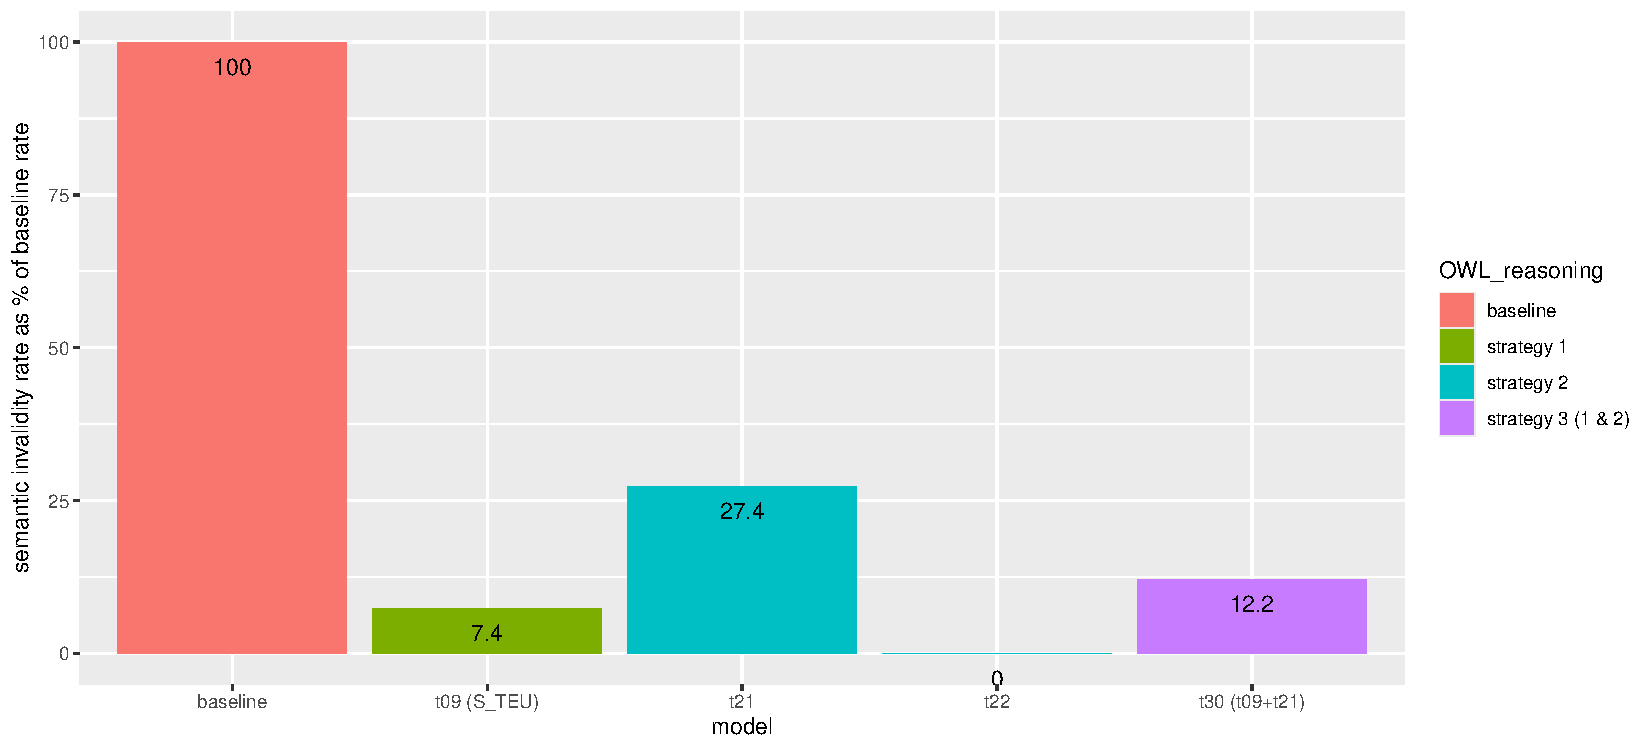
\includegraphics[width=0.9\textwidth]{figs/plot_v9_p02c-semantic-invalidity-rates_11x5.pdf}
\caption{\footnotesize A comparison of the effects of OWL reasoning strategies 1 (annotation augmentation) and 2 (prediction validation) on predictions of visual relationships that are semantically invalid, according to OWL ontology VRD-World. The scores are incidence rates of semantically invalid predictions expressed as percentages of the baseline deep learning incidence rate.}
\label{fig:nnkgs1-semantic-invalidity-rates}
\Description{A barplot showing the effects of OWL reasoning strategies 1 (annotation augmenation) and 2 (prediction validation) on the incidence rate with which semantically invalid visual relationships are predicted. The incidence rates of the neurosymbolic treatment systems are expressed as percentages of the incidence rate of the baseline system. Treatment t21 (which uses prediction validation during training) generates semantically invalid predictions at a rate just 27.4\% that of the baseline rate. Treatment t09 (which uses annotation augmentation) generates semantically invalid predictions at a rate just 7.4\% that of the baseline rate.}
\end{figure}

Recall as well that OWL reasoning strategy 2 was conceived specifically to reduce the incidence rate of semantically invalid predictions.
OWL reasoning strategy 1 (annotation augmentation), on the other hand, was conceived to improve recall@N, primarily.
Yet, as can be seen in Figure \ref{fig:nnkgs1-semantic-invalidity-rates}, treatment t09 (S\_TEU), a representative of strategy 1 (and the best performer with respect to recall@N), produces semantically invalid predictions at a rate that is only 7.4\% that of the baseline deep learning system.
In other words, OWL reasoning strategy 1 (annotation augmentation) \emph{can have} 
the useful \emph{side-effect} feature of acting like an \emph{implicit} logical constraint with respect to semantically invalid predictions.
A plausible explanation is that the logically expanded and enriched training image scene graphs produced by neurosymbolic treatment t09 (S\_TEU) are so good at helping the PPNN learn to predict semantically valid visual relationships that the incidence of semantically invalid ones diminishes in tandem.

Figure \ref{fig:nnkgs1-semantic-invalidity-rates} also shows the effects of a 3rd strategy, where OWL reasoning strategies 1 and 2 are used together, in combination.
Treatment t30 combines treatment t09 (S\_TEU), from strategy 1, with treatment t21, from strategy 2.
We see that this neurosymbolic treatment system produces semantically invalid predictions at a rate just 12.2\% that of the baseline deep learning system.
A reasonable interpretation is to say that this shows that the two OWL reasoning strategies---the two forms of logical constraints, \emph{soft} and \emph{implicit}---work together co-operatively: strategy 1 (t09) helps to make strategy 2 (the soft constraints part, at least, per t21) more effective.
A reverse interpretation is also available, however: that strategy 2 (t21) makes strategy 1 (t09) less effective.

One reason for treatment t21 (soft logical constraints applied during training) not being more effective at reducing the incidence of semantically invalid predictions may be that we do not validate predictions (or apply semantic loss penalties) unless and until the PPNN's confidence in a prediction rises above a threshold of 0.5.
It is possible for invalid predictions to cross this threshold late in a training cycle, shortly before early-stopping kicks-in, and before semantic loss penalties have had an opportunity to influence learning.
Another contributing factor may be that the value we gave to the hyperparameter that regulates the influence of our semantic loss penalties was too low.
We used a value of 1.
Larger values may be more effective, but this remains to be investigated.

Table \ref{table:semantic-validity-pvrs} shows the analysis that underlies the findings presented in Figure \ref{fig:nnkgs1-semantic-invalidity-rates}.
We can see that the incidence rates of semantically invalid predictions are naturally tiny---too tiny for any differences to be discernible in global metrics like recall@N and mAP@N.
The rate of semantic invalidity is simply the invalid count divided by the predicted count.

\begin{table}[t]
  \centering
  \footnotesize
  \begin{threeparttable}
  \caption{\footnotesize A comparison of the incidence rates of semantically invalid predicted visual relationships for treatments using OWL reasoning strategy 1 (annotation augmentation) and strategy 2 (prediction validation). The counts are calculated for topN=999 (\ie the analysis considers \emph{all} visual relationships predicted for each image).}
  \label{table:semantic-validity-pvrs}
  \begin{tabular}{clrrrrr}
    \toprule
              &     & mean  & mean  & mean  &          &   \\
              &    & total & total & total &   & \% change in \\
    OWL       &    & number & number & number & rate of & invalidity \\
    reasoning & neurosymbolic  & VRs  & VRs & VRs & semantic & rate relative \\
    strategy  & treatment & predicted & valid & invalid & invalidity & to baseline \\
              &    & (count) & (count) & (count) & (rate) & (\% chg) \\
    \midrule 
    n/a & baseline & 32101 & 32008 & 93 & 0.002904 & \\
    1  & t09 (S\_TEU) & 56071 & 56059 & 12 & 0.000214 & \textbf{-92.6}\% \\
    2  & t21 (training only) & 29427 & 29403 & 24 & 0.000795 & \textbf{-72.6}\% \\
    2  & t22 (training \& inference) & 29403 & 29403 & 0 & 0 & \textbf{-100.0}\% \\
    1 \& 2 & t30 (t09 \& t21) & 56426 & 56406 & 20 & 0.000354 & \textbf{-87.8}\% \\
    \bottomrule 
  \end{tabular}
  \end{threeparttable}
\end{table}

\subsubsection{On the volume of predictions}

\begin{figure}[t]
  \centering
  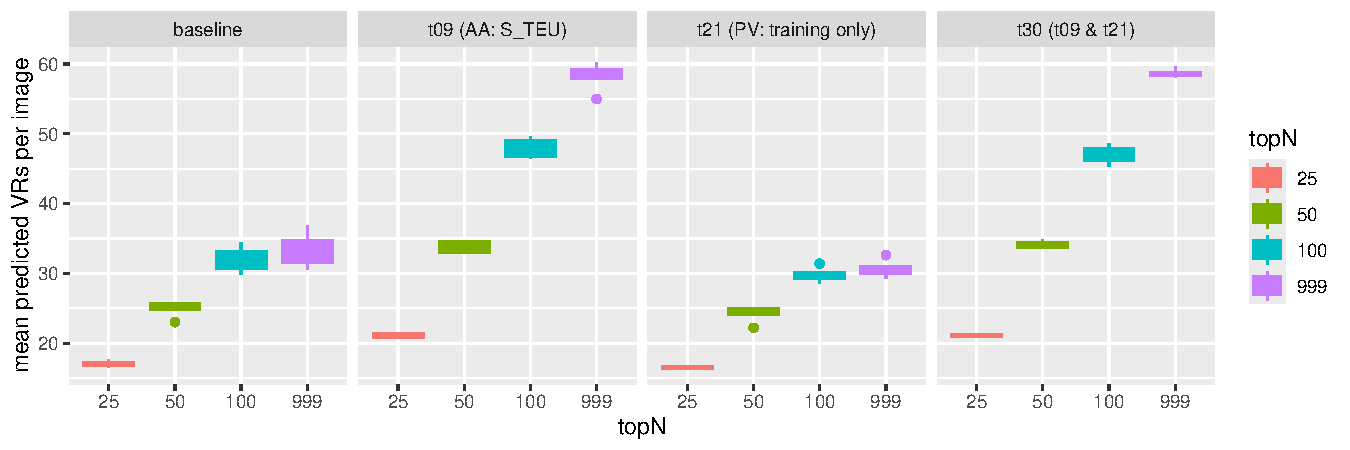
\includegraphics[width=1.0\textwidth]{figs/plot_nnkgs1_v01_p05b_RStudioExport_9x3.pdf}
  \caption{\footnotesize A comparison of the effects of OWL reasoning strategies 1 (annotation augmentation) and 2 (prediction validation) on the mean number of visual relationships predicted per image. Neurosymbolic treatment t09 uses strategy 1, treatment t21 uses strategy 2 (during training), and treatment t30 uses strategies 1 and 2, together.}
  \label{fig:nnkgs1-owl-re-on-nr-pvrs}
  \Description{A boxplot comparing the effects of OWL reasoning strategies 1 (annotation augmenation) and 2 (prediction validation) on the mean number of predicted visual relationships generated per image. The figure has four facets arranged horizontally, for systems: baseline, t09 (annotation augmentation), t21 (prediction validation) and t30 (t09 and t21 used together). For each system/facet (baseline or treatment), four boxes (distributions of scores) are plotted, one for each of the topN values of 25, 50, 100 and 999. Treatment t09 generates far more predictions per image than baseline; treatment t21 generates slightly less predictions than baseline; treatment t30 generates about the same as t09.}
\end{figure}


Figure \ref{fig:nnkgs1-owl-re-on-nr-pvrs} compares the effects of our two OWL reasoning strategies, annotation augmentation and prediction validation, on the mean number of visual relationships predicted per image. 
The effects differ dramatically.
As we saw earlier, when considering the findings for OWL reasoning strategy 1 in isolation, neurosymbolic treatment t09 (its logical expansion of the training image scene graphs) induces many more predictions of visual relationships per image.
In contrast, the semantic loss penalties, applied as soft logical constraints by treatment t21 (representing OWL reasoning strategy 2, used in training) appear to suppress predictions slightly.
For treatment t30, the combination strategy, the influence of treatment t09 (using OWL reasoning strategy 1) clearly dominates over that of treatment t21 (strategy 2).

\subsubsection{On recall@N}

\begin{figure}[t]
  \centering
  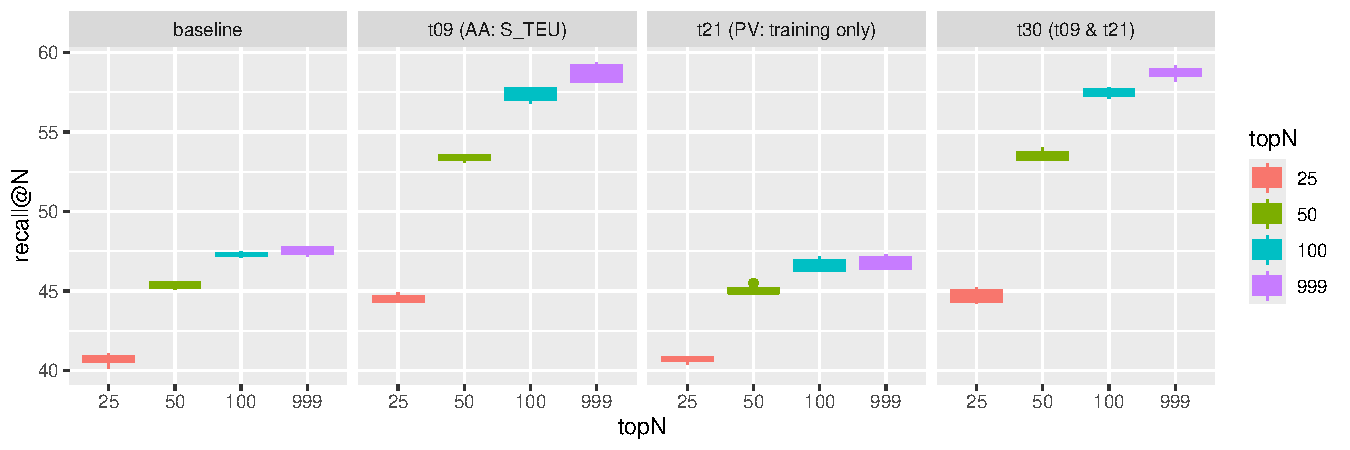
\includegraphics[width=1.0\textwidth]{figs/plot_nnkgs1_v01_p06b_RStudioExport_9x3.pdf}
  \caption{\footnotesize A comparison of the effects of OWL reasoning strategies 1 (annotation augmentation) and 2 (prediction validation) on recall@N. Neurosymbolic treatment t09 uses strategy 1, treatment t21 uses strategy 2 (during training), and treatment t30 uses strategies 1 and 2, together.}
  \label{fig:nnkgs1-owl-re-on-recall}
  \Description{A boxplot comparing the effects of OWL reasoning strategies 1 (annotation augmenation) and 2 (prediction validation) on recall@N. The figure has four facets arranged horizontally, for systems: baseline, t09 (annotation augmentation), t21 (prediction validation) and t30 (t09 and t21 used together). For each system/facet (baseline or treatment), four boxes (distributions of scores) are plotted, one for each of the topN values of 25, 50, 100 and 999. Treatment t09 has recall@N much larger than baseline; treatment t21 has recall@N slightly less than baseline; treatment t30 has recall@N about the same as t09.}
\end{figure}

Figure \ref{fig:nnkgs1-owl-re-on-recall} compares the effects of our two OWL reasoning strategies, annotation augmentation and prediction validation, on recall@N. 
Once again, the effects differ dramatically. 
Surprisingly, despite the naturally tiny incidence rates of semantically invalid predictions seen earlier, in Table \ref{table:semantic-validity-pvrs}, treatment t21's powerful reduction of the tiny incidence rate (relative to baseline) is associated with a visibly discernible effect on recall@N.
But the small dip in recall@N (relative to baseline) associated with treatment t21 is well explained by the corresponding dip in prediction volumes seen in Figure \ref{fig:nnkgs1-owl-re-on-nr-pvrs}.
Hence, the dip in recall@N appears to be a \emph{secondary} effect linked with fewer predictions, rather than a \emph{direct} effect of applying semantic loss penalties as soft logical constraints, or of there being fewer predictions of semantically invalid visual relationships.

\subsubsection{On mAP@N}

Figure \ref{fig:nnkgs1-owl-re-on-mAP} compares the effects of our two OWL reasoning strategies, annotation augmentation and prediction validation, on mAP@N.
Remember that the absolute values of our mAP@N scores are grossly pessimistic.
Recall from Table \ref{table:semantic-validity-pvrs} that treatment t21's reduction of the incidence rate of semantically invalid predictions is powerful, but that the baseline incidence rate is already tiny to begin with.
Thus, as we expected, treatment t21 does not deliver a discernible increase in mAP@N.
We can, however, discern a distinct narrowing of the variance in the distributions of mAP@N scores for treatment t21, relative to baseline.
It can only be the application of semantic loss penalties as soft logical constraints that leads to this narrowing of variance.
The mechanism by which this occurs, however, is opaque.

Observe also how, for treatment t30, which combines treatments t09 and t21 (\ie OWL reasoning strategies 1 and 2), the variance in mAP@N scores increases markedly.
This is especially the case relative to treatment t21, but it applies relative to t09 and baseline as well, although to lesser extents.
Up to now, when we have spoken of \emph{interactions}, we have referred to interactions between subcategories of OWL link inference semantics---\ie interactions that are \emph{internal} to OWL reasoning strategy 1 (annotation augmentation).
This marked increase in variance in the mAP@N scores for combination treatment t30 is an instance of a fresh category of interactions: it is evidence of an \emph{interaction} between the two OWL reasoning strategies themselves.

\begin{figure}[t]
  \centering
  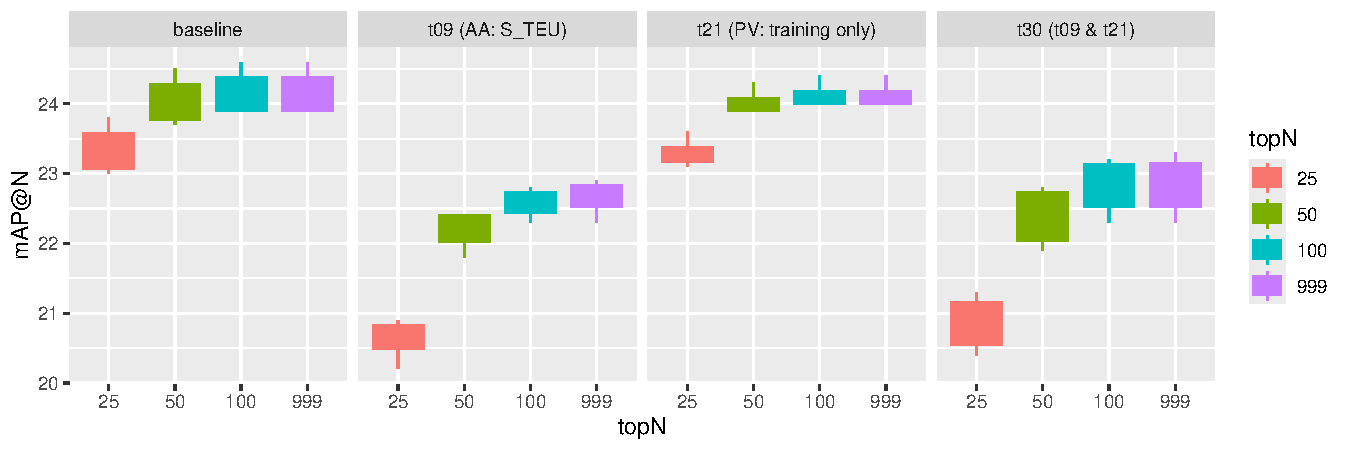
\includegraphics[width=1.0\textwidth]{figs/plot_nnkgs1_v01_p04b_RStudioExport_9x3.pdf}
  \caption{\footnotesize A comparison of the effects of OWL reasoning strategies 1 (annotation augmentation) and 2 (prediction validation) on mAP@N. Neurosymbolic treatment t09 uses strategy 1, treatment t21 uses strategy 2 (during training), and treatment t30 uses strategies 1 and 2, together.}
  \label{fig:nnkgs1-owl-re-on-mAP}
  \Description{A boxplot comparing the effects of OWL reasoning strategies 1 (annotation augmenation) and 2 (prediction validation) on mAP@N. The figure has four facets arranged horizontally, for systems: baseline, t09 (annotation augmentation), t21 (prediction validation) and t30 (t09 and t21 used together). For each system/facet (baseline or treatment), four boxes (distributions of scores) are plotted, one for each of the topN values of 25, 50, 100 and 999. Treatment t09 has mAP@N a bit lower than baseline; treatment t21 has mAP@N about the same as baseline; treatment t30 has mAP@N about the same as t09.}
\end{figure}

\subsubsection{On precision}

Table \ref{table:manual-precision-scores-I2} compares the effects of our two OWL reasoning strategies, annotation augmentation and prediction validation, on precision, as measured manually, by visual inspection of the visual relationships predicted for a small random sample of 25 NeSy4VRD test set images.
The first two rows of Table \ref{table:manual-precision-scores-I2} are repeated from Table \ref{table:manual-precision-scores}, for comparison purposes.

First, consider neurosymbolic treatment t21 (prediction validation during training).
It delivers the best standard precision overall, and better adjusted precision and FFP rate than treatment t09 (annotation augmentation).
But treatment t21 also clearly suppresses the volume of visual relationships predicted---confirming similar evidence seen earlier---and, hence, this alone may account for the better precision scores.

Next, consider treatment t30, which combines OWL reasoning strategies 1 and 2, represented by treatments t09 and t21, respectively.
This combination treatment delivers the best overall adjusted precision, the best FFP rate, it induces the most predictions, and it delivers the best overall standard recall.
These scores for treatment t30 are further strong evidence of \emph{interactions} between the two OWL reasoning strategies themselves.
In this case, the interactions appear co-operative, constructive, and mutually reinforcing.

\begin{table}[t]
  \centering
  \footnotesize
  \begin{threeparttable}
  \caption{\footnotesize A comparison of the effects of using OWL reasoning strategy 1 (annotation augmentation) and strategy 2 (prediction validation) on precision, for a small random sample of test set images. The adjusted precision scores exclude \emph{false} false positives (FFPs) from consideration. The FFP rate gives the proportion of false positives deemed, upon visual inspection, to be good predictions of visual relationships not annotated. Standard recall is hits per image over ground-truth annotations per image.}
  \label{table:manual-precision-scores-I2}
  \begin{tabular}{clrrrrrr}
    \toprule
            &       &            &            &        & mean   & \% change &   \\
    OWL     &       & mean       & mean       & mean       & predicted   & predicted & mean \\
    reasoning & neurosymbolic   & precision  & precision  &    FFP  &   VRs & VRs & recall \\
    strategy  & treatment & (standard)  & (adjusted) & rate  & per image & per image & (standard) \\
            & & (\%)   &  (\%)  & (\%) & (count) & (\% chg) & (\%) \\
    \midrule
    n/a    & baseline & 30.2  & 71.7  & 78.1 & 11.9 &  & 47.4 \\
    1 & t09 (S\_TEU) & 21.2  & 65.9  & 82.8 & 18.4 & 53.8 & 50.9 \\
    2 & t21 (train only) & \textbf{31.9}  & 77.6  & 84.9 & 11.5 & -03.4 & 47.7 \\
    1 \& 2 & t30 (t09+t21) & 21.7 & \textbf{79.4} & \textbf{90.9} & \textbf{18.8} & \textbf{57.9} & \textbf{51.8} \\
    \bottomrule 
  \end{tabular}
  \end{threeparttable}
\end{table}



% = = = = = = = = = = = = = = = = = = = = = = = = = = = = = = = = = = 



\section{Conclusions}
\label{sec:summary}

\subsection{Summary}
We have examined the use of OWL-based knowledge graph reasoning to guide and constrain subsymbolic learning in neurosymbolic systems.
The setting was the computer vision task of detecting visual relationships in images.
Our NeSy4VRD dataset, with its companion, custom-designed, common sense OWL ontology, VRD-World, underpinned all of our investigations.
We described our baseline deep learning visual relationship detection system, and explained how we cancel the noise of object detection in order to focus exclusively on the predicate detection aspect of visual relationship detection.

We described two strategies, named \emph{annotation augmentation} and \emph{prediction validation}, for leveraging OWL reasoning in co-operation with the baseline deep learning system, thus transforming it into different incarnations of neurosymbolic systems. 
We explained how OWL reasoning strategy 1, annotation augmentation, uses OWL link inference semantics and OWL reasoning, to logically expand the training image scene graphs used to supervise the (subsymbolic) learning of the predicate detector (PPNN) component of our visual relationship detection system.
We explained how OWL reasoning strategy 2, prediction validation, uses OWL type inference and logical consistency checking capabilities to (symbolically) classify predicted visual relationships as semantically valid or invalid, so that logical constraints (soft or hard) can be applied to reduce or eliminate the latter.

Observe the contrasting characters of these two OWL reasoning strategies.
Strategy 1 (annotation augmentation) can be said to have a \emph{positive} character: OWL reasoning infers more examples of semantically valid visual relationships, and so helps the predicate detector (deep learning) learn what \emph{to} predict: semantically valid visual relationships.
Strategy~2 (prediction validation), on the other hand, can be said to have a \emph{negative} character: it applies logical constraints to help the predicate detector learn what \emph{not to} predict: semantically invalid visual relationships.

We examined the effects of these two OWL reasoning strategies, on guiding and constraining the subsymbolic learning of the PPNN, in relation to two axes.
One axis consisted of a variety of different neurosymbolic \emph{treatment} systems, each one representing a particular configuration or form of applying one or other of the two OWL reasoning strategies.
The other axis consisted of a variety of different performance metrics, each one providing a different lens through which to probe for effects of OWL reasoning on subsymbolic (PPNN) learning.

\subsection{Contributions}
From one perspective, our findings are conditional upon the particularities of the setting of our research.
The key factors here are: \textit{(i)} the nature of the NeSy4VRD dataset, and the particular distribution of the visual relationships annotated for its images, including the relative frequencies of its 71 different predicates, both overall, and with respect to different ordered pairs of different object types, \textit{(ii)} our custom-designed, common sense OWL ontology, VRD-World, and \textit{(iii)} our choice of architecture for our predicate detector (our PPNN).
But many aspects of our research generalise beyond our particular setting, and well beyond the task of visual relationship detection.
To help make this clear, here we highlight the principles that our methods and findings illustrate, and the contributions they represent. 
We make the following observations:

\begin{itemize}
    \item Our research shows that neurosymbolic systems that leverage external, symbolic, OWL-based knowledge graph reasoning can outperform a baseline deep learning system across a range of different performance metrics. It shows that integrating OWL reasoning can deliver \emph{better} subsymbolic learning (more predictions, better recall@N, remarkably robust mAP@N and precision, more symmetric pairs, more inverse pairs, fewer semantically invalid predictions), and \emph{faster} subsymbolic learning (\ie fewer training epochs).
    \item Our research explores the effects on subsymbolic learning of different combinations of OWL reasoning capabilities, and these effects reveal much evidence of \emph{interactions} between the different inference capabilities. With respect to OWL reasoning strategy~1 (annotation augmentation), our research reveals powerful interactions between subcategories of OWL link inference semantics when they are used together in various combinations. Many interactions appear to be co-operative, constructive, and mutually reinforcing---delivering powerful boosts to the performance of neurosymbolic systems relative to baseline deep learning. Some combinations (\eg those involving the inference semantics of inverses) exhibit interactions that appear to be destructive or counter-productive. These findings show it is not simply the case that `more logical inference (more OWL reasoning) is better'. Our research also reveals interactions between the two different OWL reasoning strategies themselves: annotation augmentation and prediction validation. A neurosymbolic system that employs both strategies, together, is shown to outperform neurosymbolic systems using one or the other strategy, alone.
    \item Our research addresses the challenges posed by datasets that are not annotated exhaustively. Precision-related metrics assume exhaustive annotation, so when false positives cannot be identified reliably (as with non-exhaustive annotation), these metrics are unable to compute scores whose absolute values are meaningful. Our research demonstrates that meaningful information with respect to precision (\eg mAP@N) can, nonetheless, be obtained by observing relative changes in the (otherwise non-meaningful) absolute value scores generated by different systems. We introduce a novel metric called `adjusted precision' that excludes what we call \emph{false} false positives (FFPs) from the precision computation. We also introduce a novel metric we called the `FFP rate', which measures the proportion of false positives (FPs) that, upon visual inspection, are deemed to be good predictions of things not annotated.
    \item Our research expands applications of Semantic Web, OWL-based knowledge graph technologies by demonstrating their use as a \emph{symbolic reasoning engine} in neurosymbolic systems, and where an OWL ontology is used in a manner akin to a logic program. It demonstrates use of this OWL-based symbolic reasoning engine in batch-mode and real-time, and during neural network training as well as inference.
    \item Our research demonstrates an OWL-based symbolic reasoning engine being used as a real-time \emph{symbolic reasoning binary classifier}, to help train and constrain a neural network (subsymbolic) classifier (our predicate detector).
    \item Our research introduces a Semantic Web-based variant of the `loss-based logical constraints' approach to neurosymbolic AI. In this respect, it illustrates OWL reasoning driving the application of \emph{explicit} logical constraints, in order to guide and constrain subsymbolic learning. The explicit logical constraints are both soft (\eg semantic loss penalties, during training) and hard (\eg filtering, during inference). Our research also introduces the notion of an \emph{implicit} logical constraint (\eg the unexpected side-effect of annotation augmentation---of powerfully suppressing predictions of visual relationships that are semantically invalid). 
    \item Our research demonstrates the transfer of common sense, background knowledge from the symbolic realm of an OWL-based knowledge graph hosting an OWL ontology (\eg our symbolic reasoning engine) to the subsymbolic realm of a neural network (\eg our predicate detector).
    \item Our research demonstrates an OWL ontology controlling (causally determining) the performance delivered by a neural network trained under its influence (\eg recall@N scores respond characteristically to particular logical expansions of image scene graphs used to supervise the subsymbolic learning of our predicate detector).
    \item Our research demonstrates that real-time symbolic OWL reasoning can be integrated in neurosymbolic systems with acceptable impact on processing times, especially when used in combination with an efficient cache playing the role of memory.  Apart from being practical, this mimics human cognitive behaviour. If we reason something (\eg $7 \times 6 = 42$), we often commit the result to memory. When we need the result again, we recall it from memory rather than re-reason it. The mind leverages memory so as to use reasoning---slow, `System 2' thinking, per \citet{Kahneman2011}---sparingly.  Our research applies this pattern, and exhibits 3-way inter-operation between learning, reasoning, and memory---co-operation that eliminates redundant reasoning.
\end{itemize}

\subsubsection{Reusable patterns underlie our methods}
Observe also that several aspects of our methods for leveraging OWL reasoning are instances of generic patterns: \emph{(i)} the use of a \emph{custom} OWL ontology, well-aligned with the domain of interest---so that logical inference outcomes are pertinent to the learning task at hand; \emph{(ii)} the exercising of OWL \emph{link} inference capabilities to infer new knowledge---knowledge that takes the form of new links between existing individuals; \emph{(iii)} the declaration of ontological constraints, in our case using property domain/range restrictions with class disjointness; and \emph{(iv)} the leveraging of OWL \emph{type} inference capabilities, \eg for inferring exhaustive class membership for individuals.
All of these patterns, and more, can be adapted to and exploited within OWL-based neurosymblic system contexts generally.

\subsubsection{OWL-based knowledge graphs can deliver logical constraints at scale}
Lastly, we describe a contribution of our research that is highly relevant to the issue of \emph{scalability} with respect to `loss-based logical constraints' approaches to neurosymbolic AI.
\citet{DBLP:conf/ijcnn/DonadelloS19} explore visual relationship detection on the VRD dataset \cite{lu2016visual} using Logic Tensor Networks (LTN) \cite{DBLP:conf/nesy/SerafiniG16,DBLP:journals/ai/BadreddineGSS22}.
They use LTN \emph{Real Logic} knowledge axioms to declare \emph{negative} domain and \emph{negative} range constraints for relevant VRD dataset predicates.
For example, to train a binary classifier for predicate \texttt{wear}, they declare many negative domain LTN \emph{Real Logic} axioms (constraints), such as 
\begin{displaymath}
  \forall x y \ wear(x, y) \rightarrow \lnot Laptop(x), \quad 
  \forall x y \ wear(x, y) \rightarrow \lnot Sofa(x), \quad 
  \dots \ ,
\end{displaymath}
and they declare many negative range LTN \emph{Real Logic} constraints, such as
\begin{displaymath}
  \forall x y \ wear(x, y) \rightarrow \lnot Table(y), \quad 
  \forall x y \ wear(x, y) \rightarrow \lnot Car(y), \quad 
  \dots \ .
\end{displaymath}
They implement only a \emph{tractable sample} of the constraint axioms implied by their strategy, however, because the 100 object classes and 70 predicates of the VRD dataset lead to a combinatorial explosion in the number of constraint axioms requiring expression.

Our OWL reasoning strategy 2 (prediction validation)---when used during training, to apply semantic loss penalties as soft logical constraints to suppress semantically invalid visual relationships---can be viewed as an OWL-based knowledge graph counterpart of the \citet{DBLP:conf/ijcnn/DonadelloS19} LTN-based approach to visual relationship detection.
We, however, encountered no tractability issues whatsoever, and were not forced to make compromises---and our NeSy4VRD dataset has 109 object classes and 71 predicates.

One part of the explanation for this, we believe, has to do with OWL class hierarchies, and the efficiencies they enable with respect to describing domains.
General classes (at higher levels in a hierarchy)---ones that subsume many dataset classes---can permit domains to be described (and constraints expressed, or rules defined) with greater parsimony than might otherwise be feasible, if forced to express all constraints using only granular dataset classes.
Another part of the explanation is that, with an OWL ontology, and OWL reasoning, instead of expressing many \emph{negative} domain and range constraints, it was sufficient for us to express relatively few \emph{positive} domain and range restrictions.
For example, for VRD-World property (predicate) \texttt{vrd:wear}, all we had to do was declare axioms \texttt{vrd:wear rdfs:domain vrd:WearCapableThing} and \texttt{vrd:wear rdfs:range vrd:WearableThing}, and declare the two classes to be disjoint, with axiom \texttt{vrd:WearCapableThing owl:disjointWith vrd:WearableThing}.
The approach used by \citet{DBLP:conf/ijcnn/DonadelloS19} would have required nearly 200 LTN \emph{Real Logic} constraints (like the examples above) to express logically equivalent symbolic background knowledge.
In other words, our research demonstrates that our OWL-based knowledge graph variant of the `loss-based logical constraints' approach to neurosymbolic AI appears to scale well.

\subsection{Future work}

Here we briefly discuss some potential avenues of future work.

\subsubsection{Proactive prediction evaluation}

Consider OWL reasoning strategy 2 (prediction validation), used during the training of our predicate detector.  
This represents a \emph{reactive} use of OWL reasoning, and a \emph{reactive} application of loss penalties as (soft) logical constraints.
We wait for the network's confidence in a prediction to rise above a probability threshold of 0.5 before using our symbolic reasoning binary classifier to validate that (emerging) prediction of a visual relationship.

\begin{figure}
  \center
  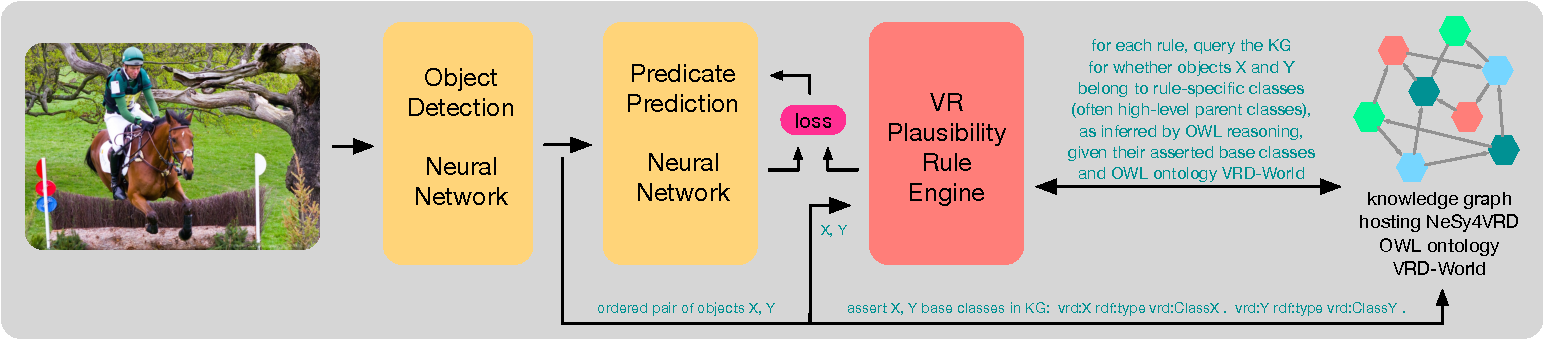
\includegraphics[width=1.0\textwidth]{figs/NN+KG-Strategy-S2-A-1-v2.pdf}
  \caption{\footnotesize A vision of an OWL-based neurosymbolic visual relationship detection system that uses Datalog-like rules, executed in a rule engine, together with OWL-based knowledge graph reasoning and queries, to \emph{proactively} scan the prediction space of a neural network, in order to identify logically plausible and logically implausible visual relationship predictions. Predictions of logically implausible visual relationships attract a logical constraint penalty, to discourage their prediction. Predictions that fail to emerge for logically plausible visual relationships attract a logical inducement penalty, to encourage the network to learn to make these high-value (likely-to-be-a-hit) visual relationships.}
  \label{fig:nn-kg-s2-setting}
  \Description{An illustration of a neurosymbolic visual relationship detection system designed to investigate the idea of \emph{proactive prediction evaluation}, where the entire prediction space of our predicate detector will be evaluated. Here, a rule engine for executing Datalog-like rules (that extend OWL's inference capabilities) mediates the interaction between the predicate detector and the OWL-based knowledge graph. The predicate detector feeds ordered pairs of objects into the rule engine, and the rule engine executes its set of rules for each ordered pair of objects. Queries to the knowledge graph are needed to check whether certain rule goals are satisfied or not. If a rule infers that a certain relationship is plausible, but the predicate detector shows no signs of learning it, we can apply a logical inducement penalty, to prompt the network to learn that prediction.}
\end{figure}

In contrast, one potential avenue for future work involves exploring the \emph{proactive} use of OWL reasoning to help guide and constrain subsymbolic learning.
More specifically, we think it feasible to logically scan (proactively logically evaluate) the entire prediction space of our predicate detector, in order to pre-identify visual relationships that are \textit{(i)} logically plausible (and, hence, should probably be predicted, because they are potential hits), and \textit{(ii)} logically implausible (and, hence, should not be predicted, because they are unlikely to be hits).
This way, we can apply logical \emph{inducement} penalties whenever a visual relationship deemed to be logically plausible is not being predicted by the network, and we can apply logical \emph{constraint} penalties whenever a visual relationship deemed to be logically implausible is being predicted by the network.
Figure \ref{fig:nn-kg-s2-setting} shows the vision for this research setting.

Datalog-like rules describing visual relationships execute in a rule engine.
For example, here is a potential rule for the visual relationship pattern \texttt{(x wear y)}:
\begin{verbatim}
    wear(x,y) :- WearCapableThing(x), WearableThing(y), ir(y,x) ~ 1.
\end{verbatim}
Prior to execution of the rules, the dataset classes (predicted or annotated) for the objects involved in an ordered pair, (X, Y), are asserted within an OWL-based knowledge graph hosting OWL ontology VRD-World.
OWL \emph{type} inference then infers all of their parent classes.
When a rule executes, the knowledge graph is queried to check if the class-specific goals of the rule are satisfied or not. 
If all goals are satisfied, that visual relationship (for that specific ordered pair of objects) is deemed logically plausible.
Otherwise, it is deemed logically implausible.
(In the example rule, above, the third goal is an \emph{inclusion ratio} condition on the bounding boxes of the two objects.)

\subsubsection{Symbolic supplementary features}
Recall that in Section \ref{sec:methods}, we explained that, to help our predicate detector learn, its core input features---the classes and the bounding boxes of ordered pairs of objects---are supplemented with geometric and spatial features derived from the bounding boxes (\eg inclusion ratios).
Another potential avenue for future work involves migrating the supplementary background knowledge from being represented as continuous input features to being represented discretely and symbolically, within an OWL-based knowledge graph hosting a (suitably extended) version of OWL ontology VRD-World.
The value and influence of the supplementary background knowledge on subsymbolic learning would be obtained via real-time OWL reasoning, governed by VRD-World, over the symbolically represented geometric and spatial features.

\subsubsection{Making soft constraints harder}
In OWL reasoning strategy 2 (prediction validation), during predicate detector training, the hyper-parameter controlling the influence of our semantic loss penalties was given the value $\lambda=1$.
The hypothesis is that larger values should make these soft logical constraints harder, and hence more effective at suppressing semantically invalid predictions.
Preliminary experiments, however, revealed $\lambda=10$ to be less effective, not more effective.
A package of work is called for involving a systematic grid search over values for $\lambda$ in order to find the range of effective values, and its sweet spot, and to discover why it is not simply the case that larger values are more effective.



% = = = = = = = = = = = = = = = = = = = = = = = = = = = = = = = = = = 




%%
%% The acknowledgments section is defined using the "acks" environment
%% (and NOT an unnumbered section). This ensures the proper
%% identification of the section in the article metadata, and the
%% consistent spelling of the heading.
%\begin{acks}
%To Robert, for the bagels and explaining CMYK and color spaces.
%\end{acks}

%%
%% The next line prints the references.
\printbibliography


%%
%% If your work has an appendix, this is the place to put it.
\appendix


\section{Online Resources}

\noindent
\textbf{Source code for our experiments}: \url{https://github.com/djherron/KGR4VRD}

\noindent
\textbf{NeSy4VRD dataset package}: \url{https://doi.org/10.5281/zenodo.7916355}

\noindent
\textbf{NeSy4VRD extensibility support and documentation}: \url{https://github.com/djherron/NeSy4VRD}



\section{Reproducibility Checklist for JAIR}

Select the answers that apply to your research -- one per item. 

\subsection*{All articles:}

%\hh{revised for stylistic consistency:}
\begin{enumerate}
    \item All claims investigated in this work are clearly stated. 
    [yes]
    \item Clear explanations are given how the work reported substantiates the claims. 
    [yes]
    \item Limitations or technical assumptions are stated clearly and explicitly. 
    [yes]
    \item Conceptual outlines and/or pseudo-code descriptions of the AI methods introduced in this work are provided, and important implementation details are discussed. 
    [yes]
    \item 
    Motivation is provided for all design choices, including algorithms, implementation choices, parameters, data sets and experimental protocols beyond metrics.
    [yes]
\end{enumerate}

\subsection*{Articles containing theoretical contributions:}
Does this paper make theoretical contributions? 
[no] 

If yes, please complete the list below.

\begin{enumerate}
    \item All assumptions and restrictions are stated clearly and formally. 
    [yes/partially/no]
    \item All novel claims are stated formally (e.g., in theorem statements). 
    [yes/partially/no]
    \item Proofs of all non-trivial claims are provided in sufficient detail to permit verification by readers with a reasonable degree of expertise (e.g., that expected from a PhD candidate in the same area of AI). [yes/partially/no]
    \item
    Complex formalism, such as definitions or proofs, is motivated and explained clearly.
%hh: was:
%Proof sketches or intuitions are given for complex and/or novel results.
    [yes/partially/no]
    \item 
    The use of mathematical notation and formalism serves the purpose of enhancing clarity and precision; gratuitous use of mathematical formalism (i.e., use that does not enhance clarity or precision) is avoided.
    [yes/partially/no]
    \item 
    Appropriate citations are given for all non-trivial theoretical tools and techniques. 
    [yes/partially/no]
\end{enumerate}

\subsection*{Articles reporting on computational experiments:}
Does this paper include computational experiments? [yes]

If yes, please complete the list below.
\begin{enumerate}
    \item 
    All source code required for conducting experiments is included in an online appendix 
    or will be made publicly available upon publication of the paper.
    The online appendix follows best practices for source code readability and documentation as well as for long-term accessibility.
    [yes]
    \item The source code comes with a license that
    allows free usage for reproducibility purposes.
    [yes]
    \item The source code comes with a license that
    allows free usage for research purposes in general.
    [yes]
    \item 
    Raw, unaggregated data from all experiments is included in an online appendix 
    or will be made publicly available upon publication of the paper.
    The online appendix follows best practices for long-term accessibility.
    [yes]
    \item The unaggregated data comes with a license that
    allows free usage for reproducibility purposes.
    [yes]
    \item The unaggregated data comes with a license that
    allows free usage for research purposes in general.
    [yes]
    \item If an algorithm depends on randomness, then the method used for generating random numbers and for setting seeds is described in a way sufficient to allow replication of results. 
    [NA]
    \item The execution environment for experiments, the computing infrastructure (hardware and software) used for running them, is described, including GPU/CPU makes and models; amount of memory (cache and RAM); make and version of operating system; names and versions of relevant software libraries and frameworks. 
    [yes]
    \item 
    The evaluation metrics used in experiments are clearly explained and their choice is explicitly motivated. 
    [yes]
    \item 
    The number of algorithm runs used to compute each result is reported. 
    [yes]
    \item 
    Reported results have not been ``cherry-picked'' by silently ignoring unsuccessful or unsatisfactory experiments. 
    [no]
    \item 
    Analysis of results goes beyond single-dimensional summaries of performance (e.g., average, median) to include measures of variation, confidence, or other distributional information. 
    [yes]
    \item % Q13
    All (hyper-) parameter settings for 
    the algorithms/methods used in experiments have been reported, along with the rationale or method for determining them. 
    [yes]
    \item % Q14
    The number and range of (hyper-) parameter settings explored prior to conducting final experiments have been indicated, along with the effort spent on (hyper-) parameter optimisation. 
    [yes]
    \item % Q15
    Appropriately chosen statistical hypothesis tests are used to establish statistical significance
    in the presence of noise effects.
    [NA]
\end{enumerate}


\subsection*{Articles using data sets:}
Does this work rely on one or more data sets (possibly obtained from a benchmark generator or similar software artifact)? 
[yes]

If yes, please complete the list below.
\begin{enumerate}
    \item 
    All newly introduced data sets 
    are included in an online appendix 
    or will be made publicly available upon publication of the paper.
    The online appendix follows best practices for long-term accessibility with a license
    that allows free usage for research purposes.
    [yes]
    \item The newly introduced data set comes with a license that
    allows free usage for reproducibility purposes.
    [yes]
    \item The newly introduced data set comes with a license that
    allows free usage for research purposes in general.
    [yes]
    \item All data sets drawn from the literature or other public sources (potentially including authors' own previously published work) are accompanied by appropriate citations.
    [yes]
    \item All data sets drawn from the existing literature (potentially including authors’ own previously published work) are publicly available. [yes]
    %\item All data sets that are not publicly available are described in detail.
    %[yes/partially/no/NA]
    \item All new data sets and data sets that are not publicly available are described in detail, including relevant statistics, the data collection process and annotation process if relevant.
    [yes]
    \item 
    All methods used for preprocessing, augmenting, batching or splitting data sets (e.g., in the context of hold-out or cross-validation)
    are described in detail. [yes]
\end{enumerate}

\subsection*{Explanations on any of the answers above (optional):}

Per \textbf{Articles reporting on computational experiments}, Q13: Any (hyper-) parameter settings not mentioned directly in the JAIR paper are discussed in our thesis, \citet{HerronThesis2025}, to which we direct the reader for further details.

Per \textbf{Articles reporting on computational experiments}, Q14: As per Q13, our thesis contains detailed discussions of hyper-parameter optimisation exercises, and we direct the reader there for such details. 

Per \textbf{Articles reporting on computational experiments}, Q15: The majority of our results are conveyed using boxplots. The thinness of our boxes reflects an absence of variation in the distributions of the sample scores being reported. And the distances between corresponding boxes (per the vertical axes), i.e. the absence of overlap between corresponding boxes, signals the statistical significance in the shifts in the distributions of the sample scores. At first glance, Table 4 (and its extension, Table 8) might be said to benefit from reporting t-test results (p-values). But, as the text makes clear, the analysis reported in Table 4 (and 8) is \emph{supplementary} to our main experiments and results.  The analysis was conducted manually, via visual inspection, on a tiny subset of 25 images, and was designed to provide rough approximations of precision only---a glimpse into just how pessimistic and misleading are the absolute values of our mAP@N scores (due to the images having been annotated non-exhaustively).

Per \textbf{Articles using data sets}, Q6: Statistics for a significant component of our NeSy4VRD dataset (its OWL ontology, VRD-World) are provided directly in the JAIR paper. A full description of NeSy4VRD as a whole, including the annotation customisation process we undertook, and the related ontology engineering exercise we undertook to create VRD-World, are described in our NeSy4VRD paper, \citet{Herron/2023/nesy4vrd}, to which we the reader for more information.

\end{document}
\endinput
%%
%% End of file `sample-acmlarge.tex'.
